%%%%%%%%%%%%%%%%%%%%%%%%%%%%%%%%%%%%%%%%%
% Stylish Article
% LaTeX Template
% Version 2.2 (2020-10-22)
%
% This template has been downloaded from:
% http://www.LaTeXTemplates.com
%
% Original author:
% Mathias Legrand (legrand.mathias@gmail.com) 
% With extensive modifications by:
% Vel (vel@latextemplates.com)
%
% License:
% CC BY-NC-SA 3.0 (http://creativecommons.org/licenses/by-nc-sa/3.0/)
%
%%%%%%%%%%%%%%%%%%%%%%%%%%%%%%%%%%%%%%%%%
% commento per github
%----------------------------------------------------------------------------------------
%	PACKAGES AND OTHER DOCUMENT CONFIGURATIONS
%----------------------------------------------------------------------------------------

\documentclass[fleqn,10pt]{SelfArx} % Document font size and equations flushed left

%\usepackage[english]{babel} % Specify a different language here - english by default
\usepackage[italian]{babel} % Specify a different language here - english by default

\usepackage{lipsum} % Required to insert dummy text. To be removed otherwise

%----------------------------------------------------------------------------------------
%	COLUMNS
%----------------------------------------------------------------------------------------

\setlength{\columnsep}{0.55cm} % Distance between the two columns of text
\setlength{\fboxrule}{0.75pt} % Width of the border around the abstract

%----------------------------------------------------------------------------------------
%	COLORS
%----------------------------------------------------------------------------------------

\definecolor{color1}{RGB}{0,0,90} % Color of the article title and sections
\definecolor{color2}{RGB}{0,20,20} % Color of the boxes behind the abstract and headings

%----------------------------------------------------------------------------------------
%	HYPERLINKS
%----------------------------------------------------------------------------------------

\usepackage{hyperref} % Required for hyperlinks

\hypersetup{
	hidelinks,
	colorlinks,
	breaklinks=true,
	urlcolor=color2,
	citecolor=color1,
	linkcolor=color1,
	bookmarksopen=false,
	pdftitle={Title},
	pdfauthor={Author},
}

%----------------------------------------------------------------------------------------
%	ARTICLE INFORMATION
%----------------------------------------------------------------------------------------

\JournalInfo{Programmazione per l'IoT - Laurea Magistrale in Informatica Applicata - DiSPeA - Università degli Studi di Urbino Carlo Bo} % Journal information
\Archive{Data di pubblicazione xx/xx/xxxx - DOI: xxxx/xxxxxxx} % Informazioni che verranno inserite dal Docente in fase di pubblicazione

\PaperTitle{L'uso dell'IoT per la monitorazione della qualità dell'aria} % Article title

\Authors{Arlind Pecmarkaj\textsuperscript{1}*, Emanuele Lattanzi\textsuperscript{2}} % Il docente Emanuele Lattanzi figura come autore
% al fine di poter gestire la procedura di submission sul repository pubblico (nell'affiliazione viene chiarito il ruolo)
\affiliation{\textsuperscript{1}\textit{Laurea Magistrale in Informatica Applicata, Università degli Studi di Urbino Carlo Bo, Urbino, Italia}} % Author affiliation
\affiliation{\textsuperscript{2}\textit{Docente di Programmazione per l'Internet of Things, Università degli Studi di Urbino Carlo Bo, Urbino, Italia}} % Author affiliation
\affiliation{*\textbf{Corresponding author}: a.pecmarkaj@campus.uniurb.it} % Corresponding author

\Keywords{Air Quality --- Meteorology --- Internet of Things --- Machine Learning --- ESP32} % Keywords - if you don't want any simply remove all the text between the curly brackets
\newcommand{\keywordname}{Keywords} % Defines the keywords heading name

%----------------------------------------------------------------------------------------
%	ABSTRACT
%----------------------------------------------------------------------------------------

\Abstract{La qualità dell’aria rappresenta una tematica di crescente rilevanza, in particolare in diverse aree urbane e industriali del territorio italiano, dove l’esposizione prolungata a inquinanti atmosferici può avere impatti significativi sulla salute pubblica. Questo progetto si colloca nell’ambito dell’Internet of Things (IoT) e dell’analisi ambientale, con l’obiettivo di sviluppare un sistema predittivo per la qualità dell’aria basato su tecniche di machine learning. È stata realizzata una stazione meteo IoT in grado di rilevare TVOC, particolato (PM), CO2, umidità, pressione atmosferica e temperatura. I dati raccolti sono stati utilizzati per analizzare le correlazioni tra le condizioni ambientali e i livelli di inquinamento atmosferico, con particolare attenzione alla possibilità di stimare la qualità dell’aria attraverso modelli predittivi fondati unicamente su temperatura, pressione e umidità. L’approccio proposto consente di ridurre la complessità e i costi dei sistemi di monitoraggio, offrendo una soluzione scalabile e adatta a contesti distribuiti o a basso consumo, come le reti di sensori ambientali urbani.}

%----------------------------------------------------------------------------------------

\begin{document}

\maketitle % Output the title and abstract box
%\tableofcontents % Output the contents section

\thispagestyle{empty} % Removes page numbering from the first page

%----------------------------------------------------------------------------------------
%	ARTICLE CONTENTS
%----------------------------------------------------------------------------------------

\section*{Introduzione} % The \section*{} command stops section numbering
Negli ultimi anni, la crescente consapevolezza degli effetti a lungo termine dell’inquinamento atmosferico — come l’aumento delle malattie respiratorie, cardiovascolari e il peggioramento delle condizioni di vita nei centri urbani — ha reso sempre più urgente lo sviluppo di sistemi di monitoraggio capillari e a basso costo. In Italia, diverse regioni del Nord, tra cui la Pianura Padana, presentano condizioni meteorologiche e geografiche che favoriscono l’accumulo di inquinanti, rendendo ancora più evidente la necessità di sistemi intelligenti e distribuiti per il controllo della qualità dell’aria.

Tradizionalmente, il monitoraggio ambientale è stato affidato a centraline fisse, altamente precise ma costose e limitate nella copertura spaziale. L’evoluzione dell’Internet of Things (IoT) ha però aperto nuove possibilità: la miniaturizzazione dell’elettronica e la disponibilità di sensori a basso costo consentono oggi di progettare dispositivi distribuiti e intelligenti, in grado di rilevare dati ambientali in tempo reale. Tuttavia, molti sensori per la rilevazione della qualità dell’aria, come quelli per particolato (PM), composti organici volatili totali (TVOC) o biossido di carbonio (CO2), risultano energivori e poco adatti ad applicazioni di lunga durata in contesti domestici o alimentati a batteria.

In questo contesto, il presente progetto propone un approccio alternativo: l’utilizzo di tecniche di machine learning per prevedere la qualità dell’aria basandosi esclusivamente su parametri ambientali a basso consumo energetico, come temperatura, umidità e pressione atmosferica. Queste variabili, tipicamente rilevabili con sensori a basso costo e ridotto impatto energetico, sono legate alle dinamiche meteorologiche che influenzano direttamente la dispersione e l’accumulo degli inquinanti nell’atmosfera. Sebbene la correlazione non sia diretta, la modellazione statistica e predittiva consente di stimare la qualità dell’aria con un grado di affidabilità sufficiente per molte applicazioni pratiche.

L’obiettivo finale è quindi duplice: da un lato, ridurre la complessità e i consumi dei dispositivi di monitoraggio, rendendoli idonei all’installazione diffusa in ambienti domestici; dall’altro, integrare questi sistemi con attuatori intelligenti che possano intervenire automaticamente per migliorare il comfort e la salubrità degli ambienti, ad esempio regolando la ventilazione o attivando purificatori d’aria. Il tutto in un’ottica di sostenibilità, economicità e interoperabilità con le moderne tecnologie smart home

%------------------------------------------------

\section{La relazione tra variabili meteorologiche e la qualità dell’aria}
La qualità dell’aria dipende non solo dalle sorgenti emissive di inquinanti (come traffico, attività industriali o combustione domestica), ma anche dalle condizioni meteorologiche che regolano la dispersione, la trasformazione chimica e l’accumulo degli agenti inquinanti nell’atmosfera. In particolare, variabili come temperatura, umidità e pressione atmosferica, pur non essendo direttamente responsabili dell’inquinamento, rappresentano indicatori fondamentali delle dinamiche atmosferiche che condizionano la qualità dell’aria.

Le variazioni di temperatura influenzano direttamente la stabilità dell’atmosfera. Un aumento o una diminuzione repentina della temperatura può indicare il passaggio di una massa d’aria con caratteristiche fisiche differenti (fronte caldo o fronte freddo), modificando le condizioni di rimescolamento dell’aria. Temperature elevate in condizioni stabili e assenza di vento portano alla stagnazione degli inquinanti, mentre un calo improvviso della temperatura può essere sintomo di un rimescolamento verticale più attivo, che favorisce la dispersione degli stessi.
Inoltre, alte temperature estive favoriscono reazioni fotochimiche che producono ozono troposferico, un inquinante secondario che si accumula nei bassi strati atmosferici soprattutto nelle ore centrali della giornata. Le escursioni termiche tra giorno e notte, frequenti in molte zone italiane, sono quindi spesso associate a variazioni significative nei livelli di inquinamento.

L’umidità relativa gioca un ruolo cruciale nella formazione e nel comportamento del particolato atmosferico. In condizioni di elevata umidità, le particelle igroscopiche assorbono l’acqua e aumentano di dimensione, rendendosi più persistenti in atmosfera. La variazione dell’umidità può inoltre indicare la presenza di fronti in transito o di cambiamenti nella circolazione atmosferica, come l’ingresso di masse d’aria più fredde o calde, che alterano la composizione dell’aria e la sua capacità di trattenere o disperdere gli inquinanti.
Un’improvvisa diminuzione dell’umidità può ad esempio segnalare l’arrivo di aria secca e più ventilata, associata a condizioni favorevoli alla dispersione, mentre un picco di umidità in condizioni stabili può favorire la formazione di nebbie o foschie, che contribuiscono all’accumulo di inquinanti nei bassi strati.

La pressione atmosferica è un indicatore indiretto, ma molto efficace, dei processi meteorologici in atto. Un sistema di alta pressione (anticiclone) è generalmente associato a condizioni di cielo sereno, scarsa ventilazione e aria stabile — tutte situazioni favorevoli all’accumulo di inquinanti. Al contrario, un sistema di bassa pressione (ciclone) è legato a fenomeni di instabilità, venti, piogge e temporali, che contribuiscono a diluire e rimuovere gli inquinanti dall’aria.
Un repentino calo della pressione atmosferica può essere interpretato come segnale del passaggio di un fronte freddo, associato a rimescolamento turbolento, venti sostenuti e fenomeni convettivi (es. temporali estivi). Questi eventi portano a una rapida pulizia dell’aria per effetto della turbolenza meccanica e del “lavaggio” atmosferico dovuto alle precipitazioni. Anche l’aumento della pressione dopo il passaggio di un fronte può avere implicazioni: l’instaurarsi di un nuovo anticiclone può riportare rapidamente condizioni stagnanti.
Dunque, anche in assenza di sensori per il vento, le variazioni barometriche costituiscono un indizio prezioso per dedurre la ventilazione e la struttura verticale dell’atmosfera.

Le variazioni nei parametri meteorologici come temperatura, umidità e pressione non solo influenzano direttamente la qualità dell’aria, ma ne anticipano anche l’evoluzione. L’analisi delle loro tendenze temporali consente di cogliere i segnali dei cambiamenti atmosferici in atto (es. arrivo di un fronte, formazione di inversioni termiche, instabilità convettiva), che incidono significativamente sulla distribuzione e sulla concentrazione degli inquinanti. Tali variabili, se opportunamente elaborate tramite algoritmi di machine learning, possono quindi costituire un’alternativa valida alla misurazione diretta degli inquinanti.

\section{Progettazione della Stazione e Metodologia Operativa}

Il cuore del sistema di monitoraggio è un microcontrollore \textbf{ESP32}. Il firmware, sviluppato ad-hoc, orchestra l'acquisizione dei dati da una suite di sensori e la loro trasmissione a un database remoto per l'analisi.

\subsection{Componenti Hardware: Sensori e Attuatori}

La stazione è stata assemblata integrando i seguenti sensori, che comunicano con l’ESP32 tramite bus I2C e interfaccia seriale (UART):
\begin{itemize}
	\item \textbf{MH-Z19B} (via UART): Rileva la concentrazione di anidride carbonica (\texttt{CO\textsubscript{2}}) e la propria temperatura operativa.
	\item \textbf{AHT20} (via I2C): Fornisce le misurazioni primarie di temperatura e umidità relativa, usate anche per la compensazione di altri sensori.
	\item \textbf{BMP280} (via I2C): Misura la pressione atmosferica (\texttt{hPa}) e una seconda lettura di temperatura.
	\item \textbf{ENS160} (via I2C): Sensore MOX che stima l'Indice di Qualità dell’Aria (\texttt{AQI}), la \texttt{equivalent CO\textsubscript{2}} e la concentrazione di composti organici volatili totali (\texttt{TVOC}).
	\item \textbf{SPS30} (via I2C): Sensore ottico a diffusione laser che misura la concentrazione di massa di particolato (\texttt{PM1.0}, \texttt{PM2.5}, \texttt{PM4.0}, \texttt{PM10.0}) e la dimensione tipica delle particelle.
\end{itemize}

Come semplice \textbf{attuatore}, il sistema include un LED di stato per fornire un feedback visivo immediato in caso di condizioni avverse.

\subsection{Firmware: Logica di Acquisizione e Processamento Dati}

Il firmware è strutturato per garantire robustezza, efficienza e accuratezza dei dati attraverso un ciclo operativo ben definito.

\subsubsection{Fase di Avvio e Inizializzazione}
Alla prima accensione, il firmware esegue una sequenza di \textit{setup} critica:
\begin{enumerate}
	\item \textbf{Connessione di Rete:} Tenta la connessione alla rete Wi-Fi preconfigurata. In caso di successo, sincronizza l'orologio di sistema tramite NTP (\textit{Network Time Protocol}) per garantire timestamp precisi e valida la connessione al server \textbf{InfluxDB}.
	\item \textbf{Inizializzazione dei Sensori:} Viene effettuato un controllo di disponibilità (\textit{probe}) per ciascun sensore sui rispettivi bus (I2C, UART). In caso di fallimento, viene registrato un messaggio di errore, permettendo al sistema di continuare a funzionare con i sensori rimanenti.
	\item \textbf{Periodo di Riscaldamento:} Viene imposto un periodo di attesa iniziale di 60 secondi per permettere la stabilizzazione dei sensori, in particolare per i modelli MOX (ENS160) e NDIR (MH-Z19B).
\end{enumerate}

\subsubsection{Ciclo Operativo Principale}
Il sistema entra in un ciclo infinito (\textit{loop}) che si ripete ogni \textbf{5 minuti}, scandito dalle seguenti operazioni:
\begin{enumerate}
	\item \textbf{Acquisizione Dati Grezzi:} Il firmware interroga sequenzialmente tutti i sensori inizializzati.
	
	\item \textbf{Elaborazione e Validazione Dati:} I dati grezzi vengono processati per migliorarne l'affidabilità:
	\begin{itemize}
		\item \textbf{Compensazione Incrociata:} Le letture di temperatura e umidità del sensore AHT20 vengono passate al sensore ENS160 per compensarne le misurazioni.
		\item \textbf{Filtraggio dei Dati Anomali:} Vengono applicate regole di validazione per scartare letture palesemente errate o fuori range.
		\item \textbf{Calcolo della Temperatura Media:} Viene calcolata la media aritmetica delle temperature valide fornite dai sensori AHT20, BMP280 e MH-Z19B.
	\end{itemize}
	
	\item \textbf{Attuazione e Trasmissione:} In questa fase finale del ciclo, il sistema gestisce l'allerta locale e l'invio dei dati.
	\begin{itemize}
		\item \textbf{Controllo Allarmi:} Viene attivato l'\textbf{attuatore} (il LED di stato) se i dati rilevati direttamente dai sensori superano le soglie critiche, ovvero se l'\textbf{AQI fornito dal sensore ENS160} è $\ge 4$ o se il valore di \textbf{PM2.5 misurato dal sensore SPS30} è > 35.5 µg/m³.
		\item \textbf{Invio a InfluxDB:} Se la connessione Wi-Fi è attiva, i dati validati e processati vengono inviati al database. In caso contrario, la trasmissione viene saltata e il sistema tenta la riconnessione.
	\end{itemize}
\end{enumerate}

\subsection{Attuazione basata su Machine Learning}
L'attuale sistema di allerta basato su soglie dirette serve come meccanismo di feedback immediato e per la validazione dei dati. Tuttavia, l'obiettivo finale del progetto è trascendere questo approccio. La raccolta dati è finalizzata all'addestramento di un modello di \textbf{Machine Learning} che possa individuare una correlazione statisticamente significativa tra i parametri a basso consumo (temperatura, umidità e pressione) e i livelli di inquinanti (PM, TVOC, CO2).

Qualora tale correlazione venisse confermata, l'attuazione non sarebbe più legata alle soglie dei sensori diretti, ma verrebbe pilotata dal modello predittivo. Questo consentirebbe di realizzare dispositivi di monitoraggio e attuazione a costo e consumo energetico drasticamente inferiori, capaci di stimare la qualità dell'aria e, ad esempio, attivare un purificatore o un sistema di ventilazione in maniera intelligente e predittiva.



%------------------------------------------------

\section{Analisi dei dati}

Durante il periodo di rilevazione, caratterizzato dalla persistenza dell’anticiclone africano, i valori di temperatura e pressione atmosferica hanno mostrato variazioni contenute.

In Figura~\ref{fig:temperature_timeseries} si osserva l’andamento temporale della temperatura. L’unico evento anomalo è rappresentato dall’arrivo di una goccia fredda, che ha causato una temporanea diminuzione delle temperature. La distribuzione dei dati, illustrata in Figura~\ref{fig:temperature_dis}, presenta una struttura bimodale, riconducibile alle escursioni termiche giornaliere: i picchi corrispondono ai valori minimi notturni e ai massimi diurni, con un rapido riscaldamento subito dopo l’alba.

\begin{figure}[ht]\centering
	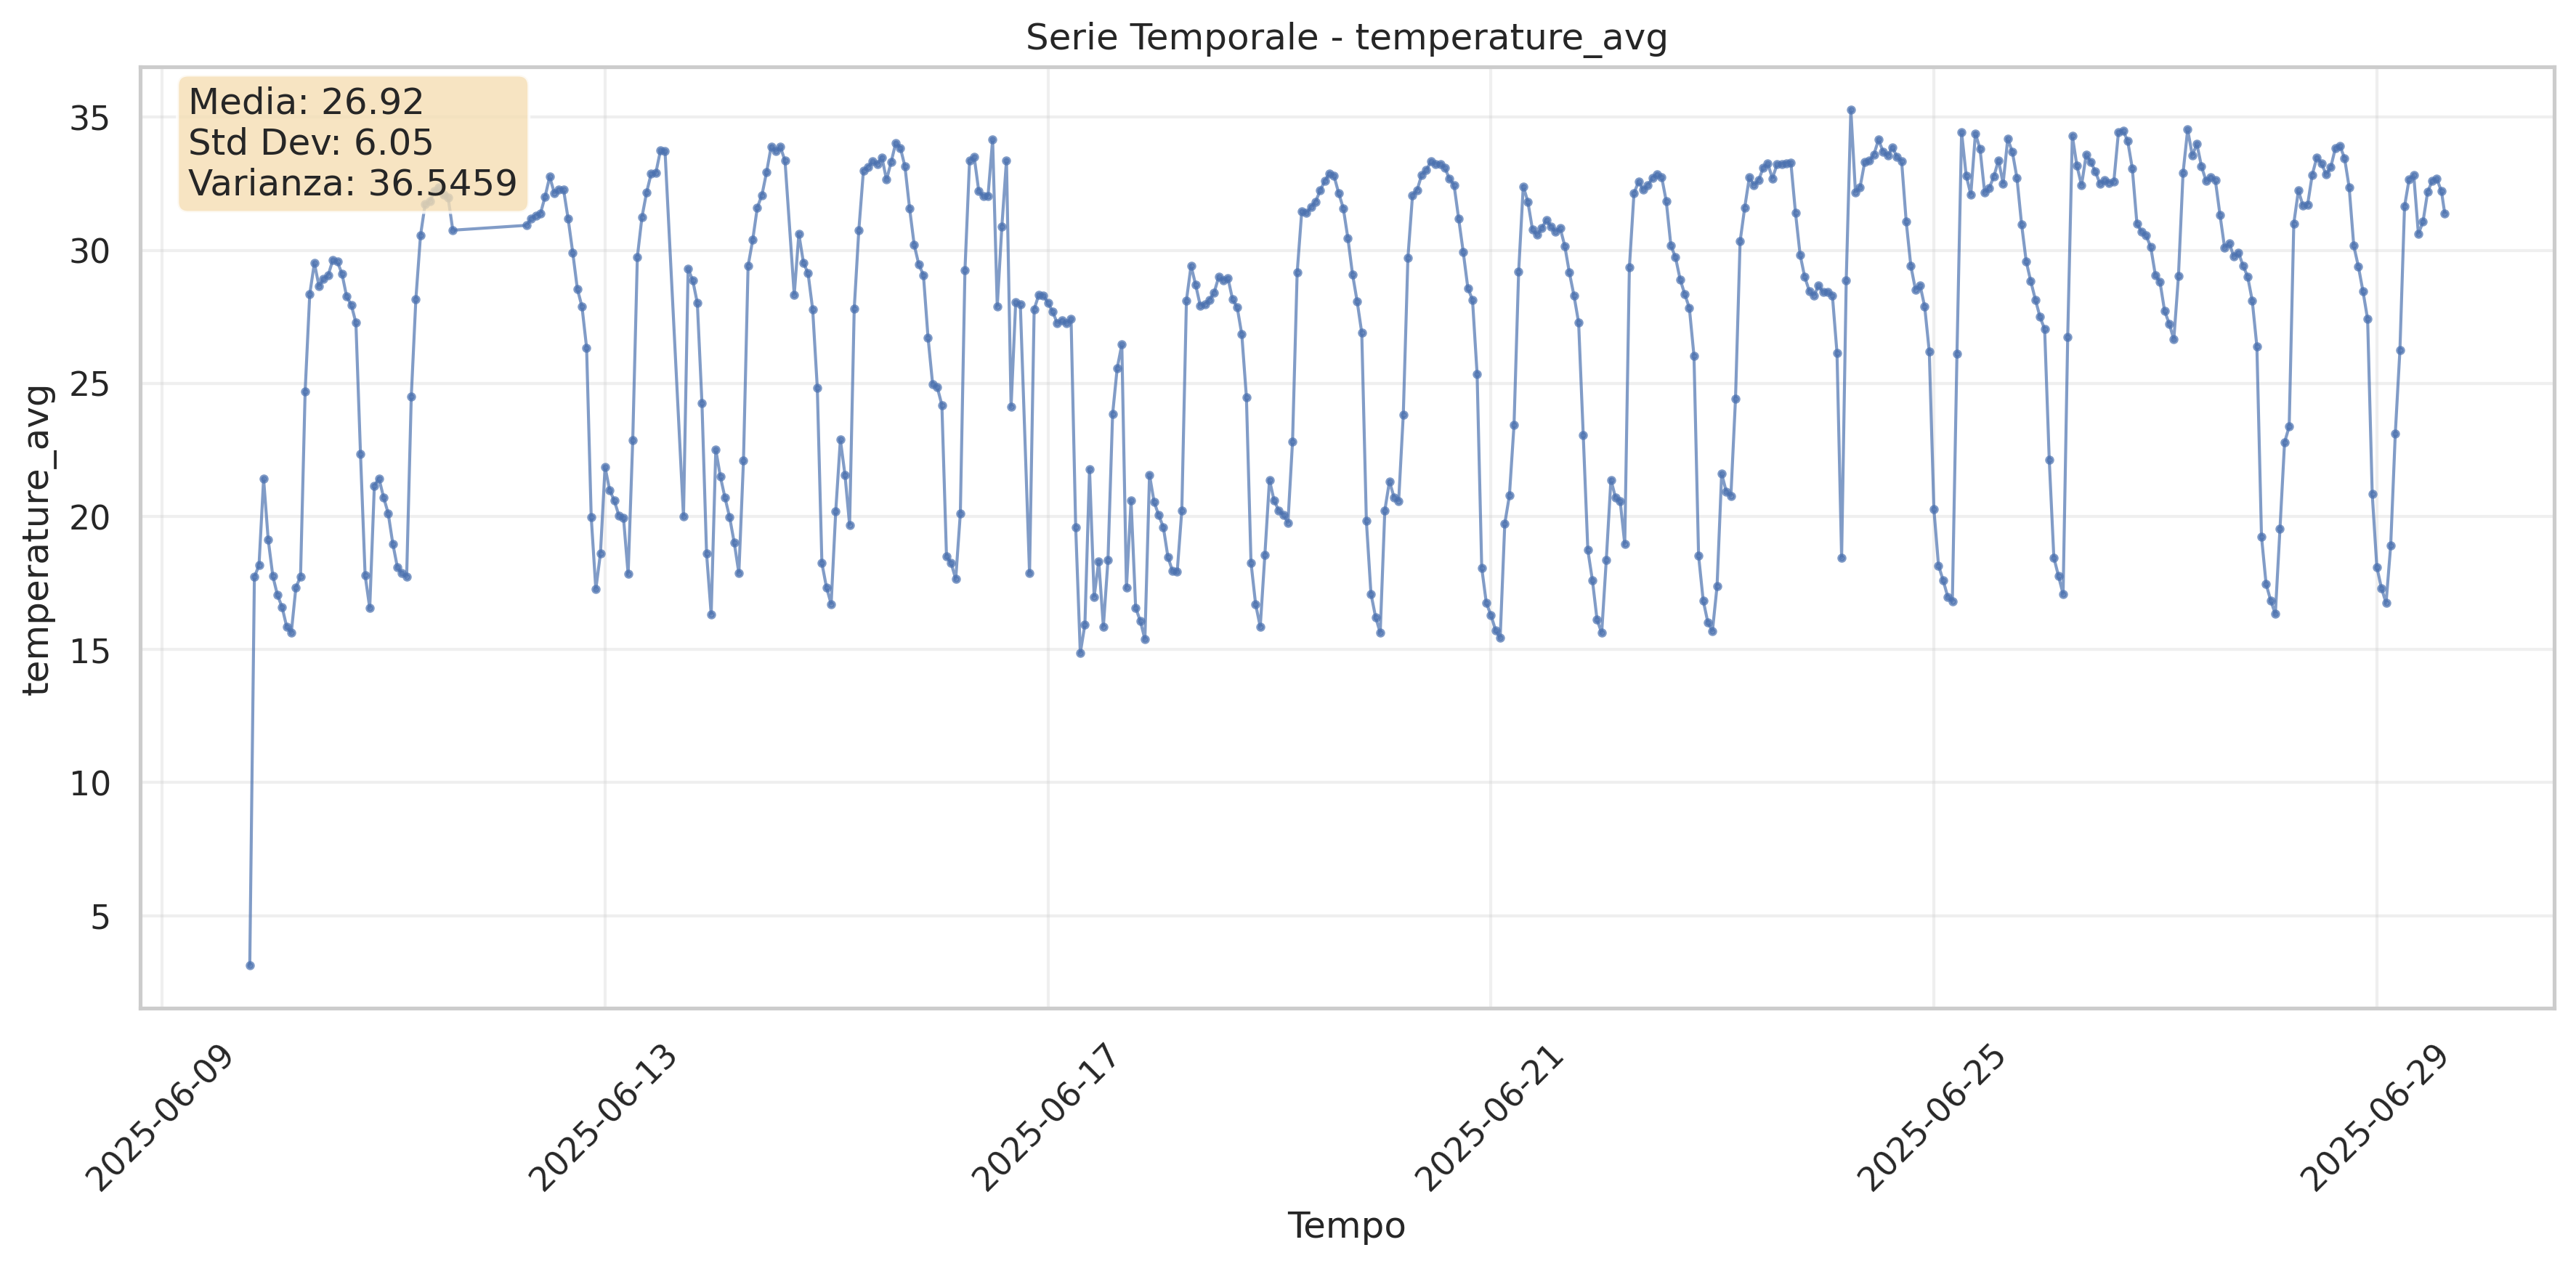
\includegraphics[width=\linewidth]{Figures/temperature_avg_timeseries}
	\caption{Andamento temporale della temperatura}
	\label{fig:temperature_timeseries}
\end{figure}

\begin{figure}[ht]\centering
	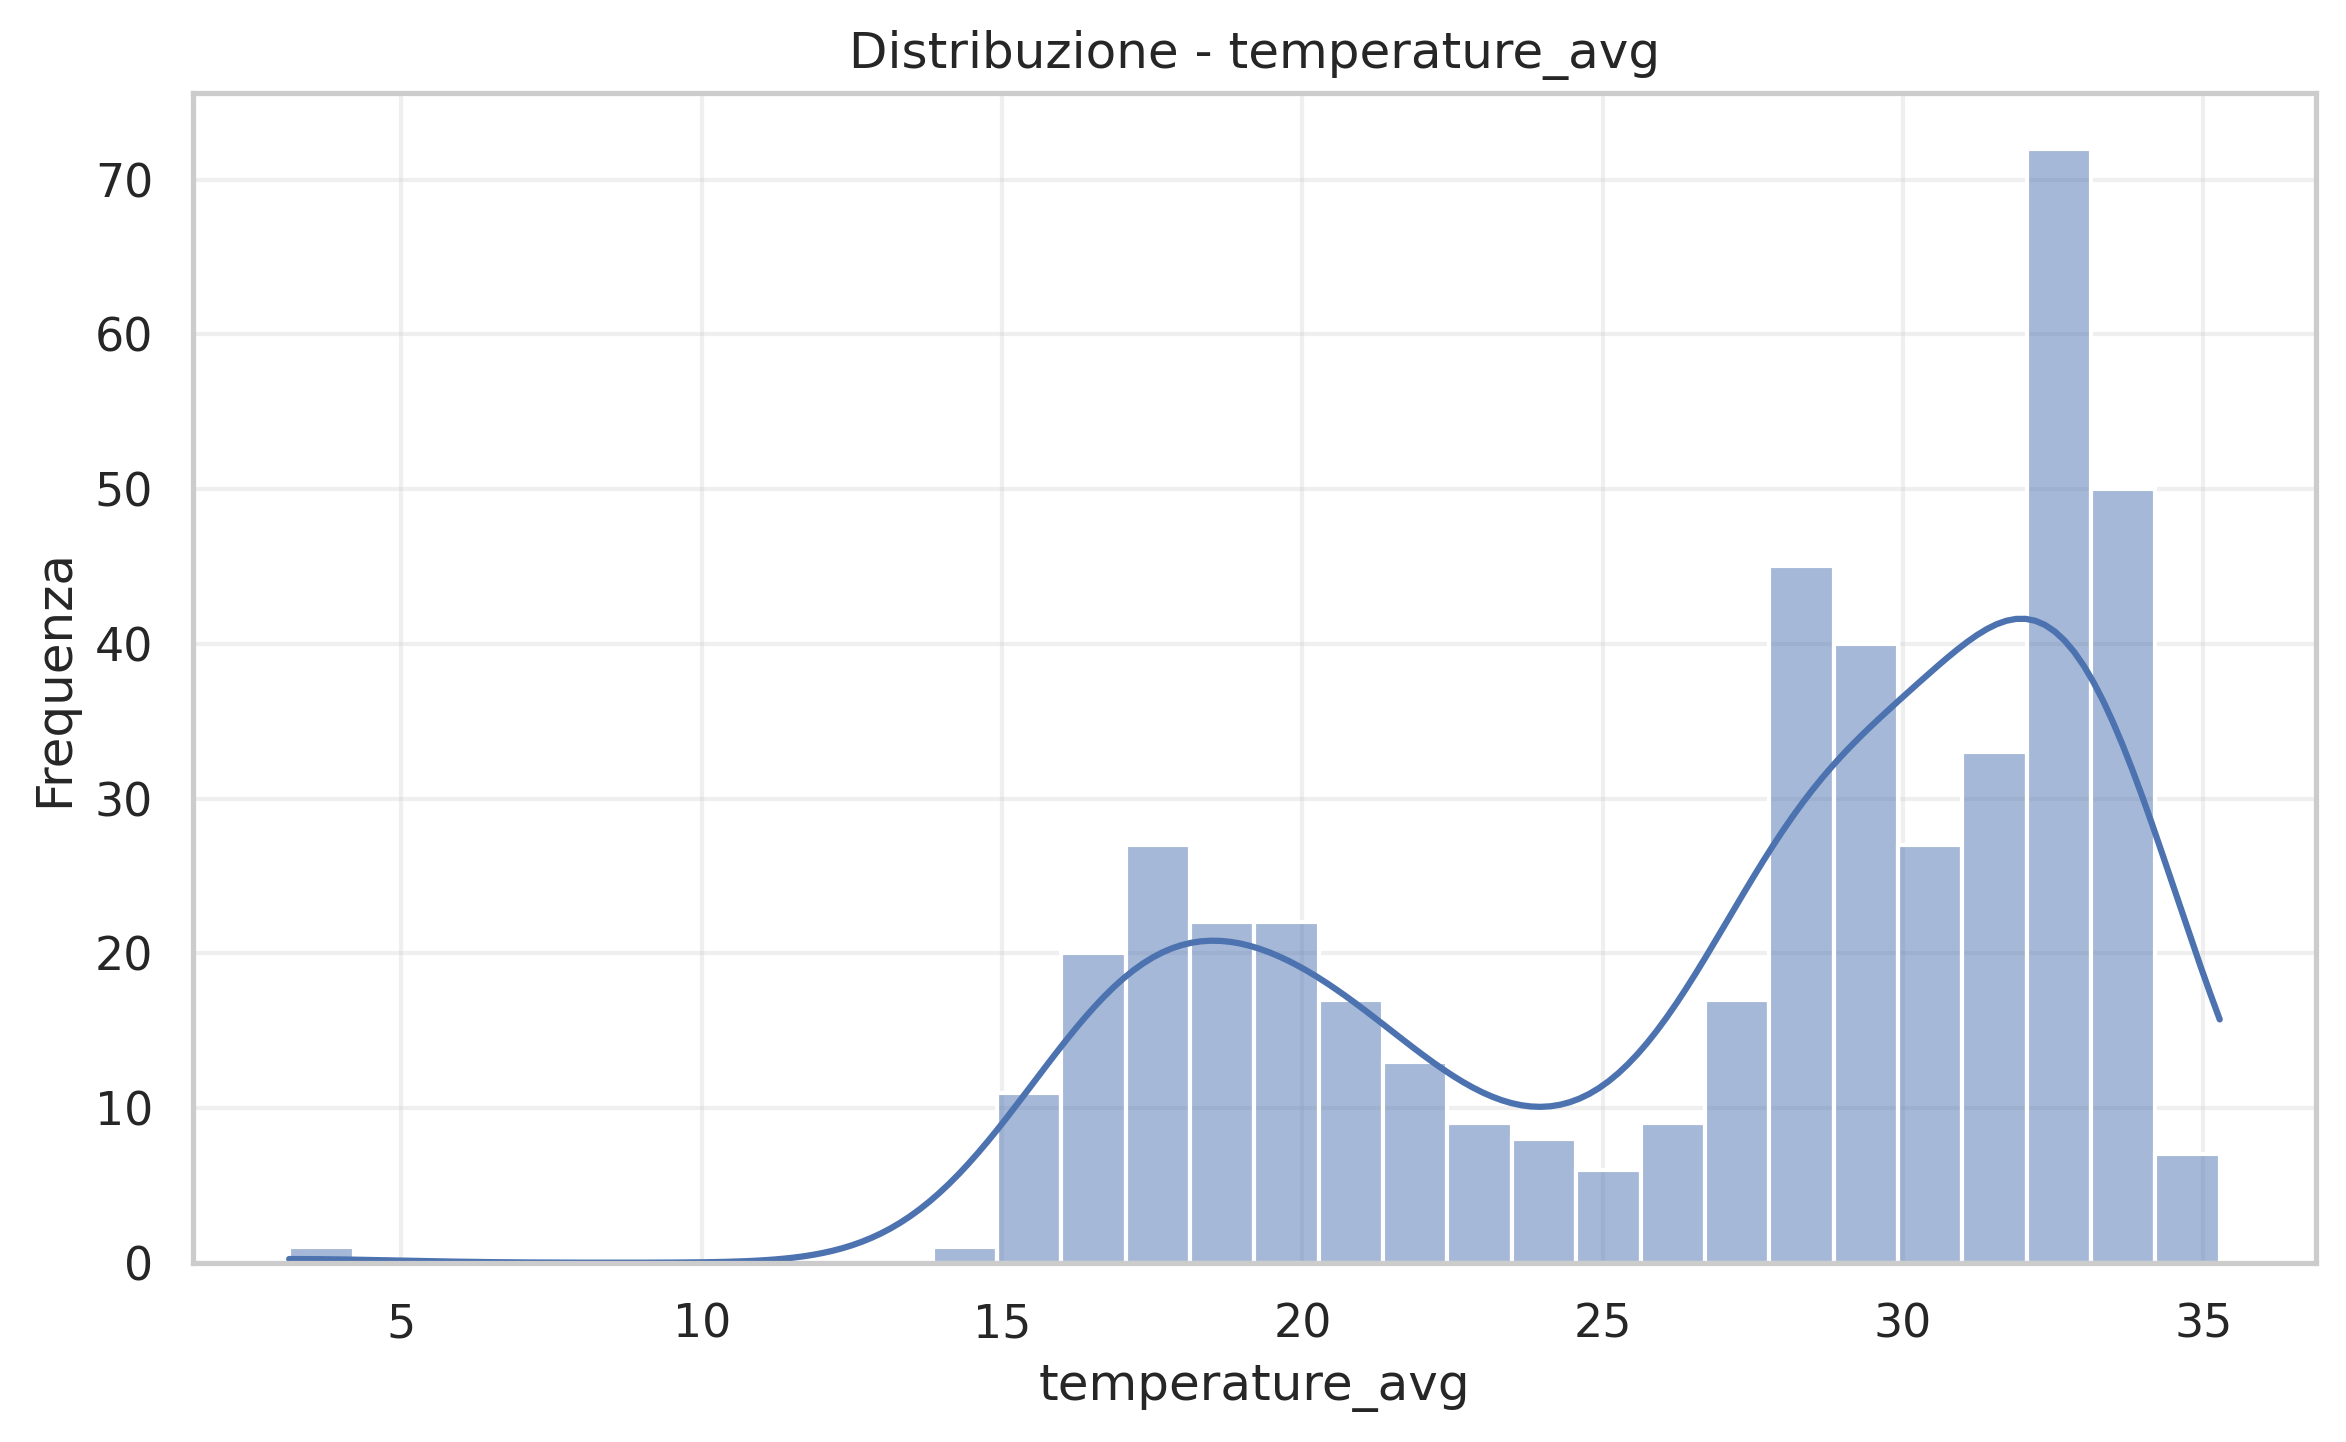
\includegraphics[width=\linewidth]{Figures/temperature_avg_distribution}
	\caption{Distribuzione della temperatura}
	\label{fig:temperature_dis}
\end{figure}

La pressione atmosferica ha mantenuto valori stabili per gran parte del periodo. Tuttavia, come mostrato in Figura~\ref{fig:pressure_timeseries}, si nota una leggera diminuzione verso la fine della rilevazione, coincidente con il consolidamento dell’anticiclone e un riscaldamento più omogeneo dell’aria. La distribuzione corrispondente (Figura~\ref{fig:press_dis}) conferma una leggera tendenza bimodale, con prevalenza di valori più bassi nella seconda parte della campagna.

\begin{figure}[ht]\centering
	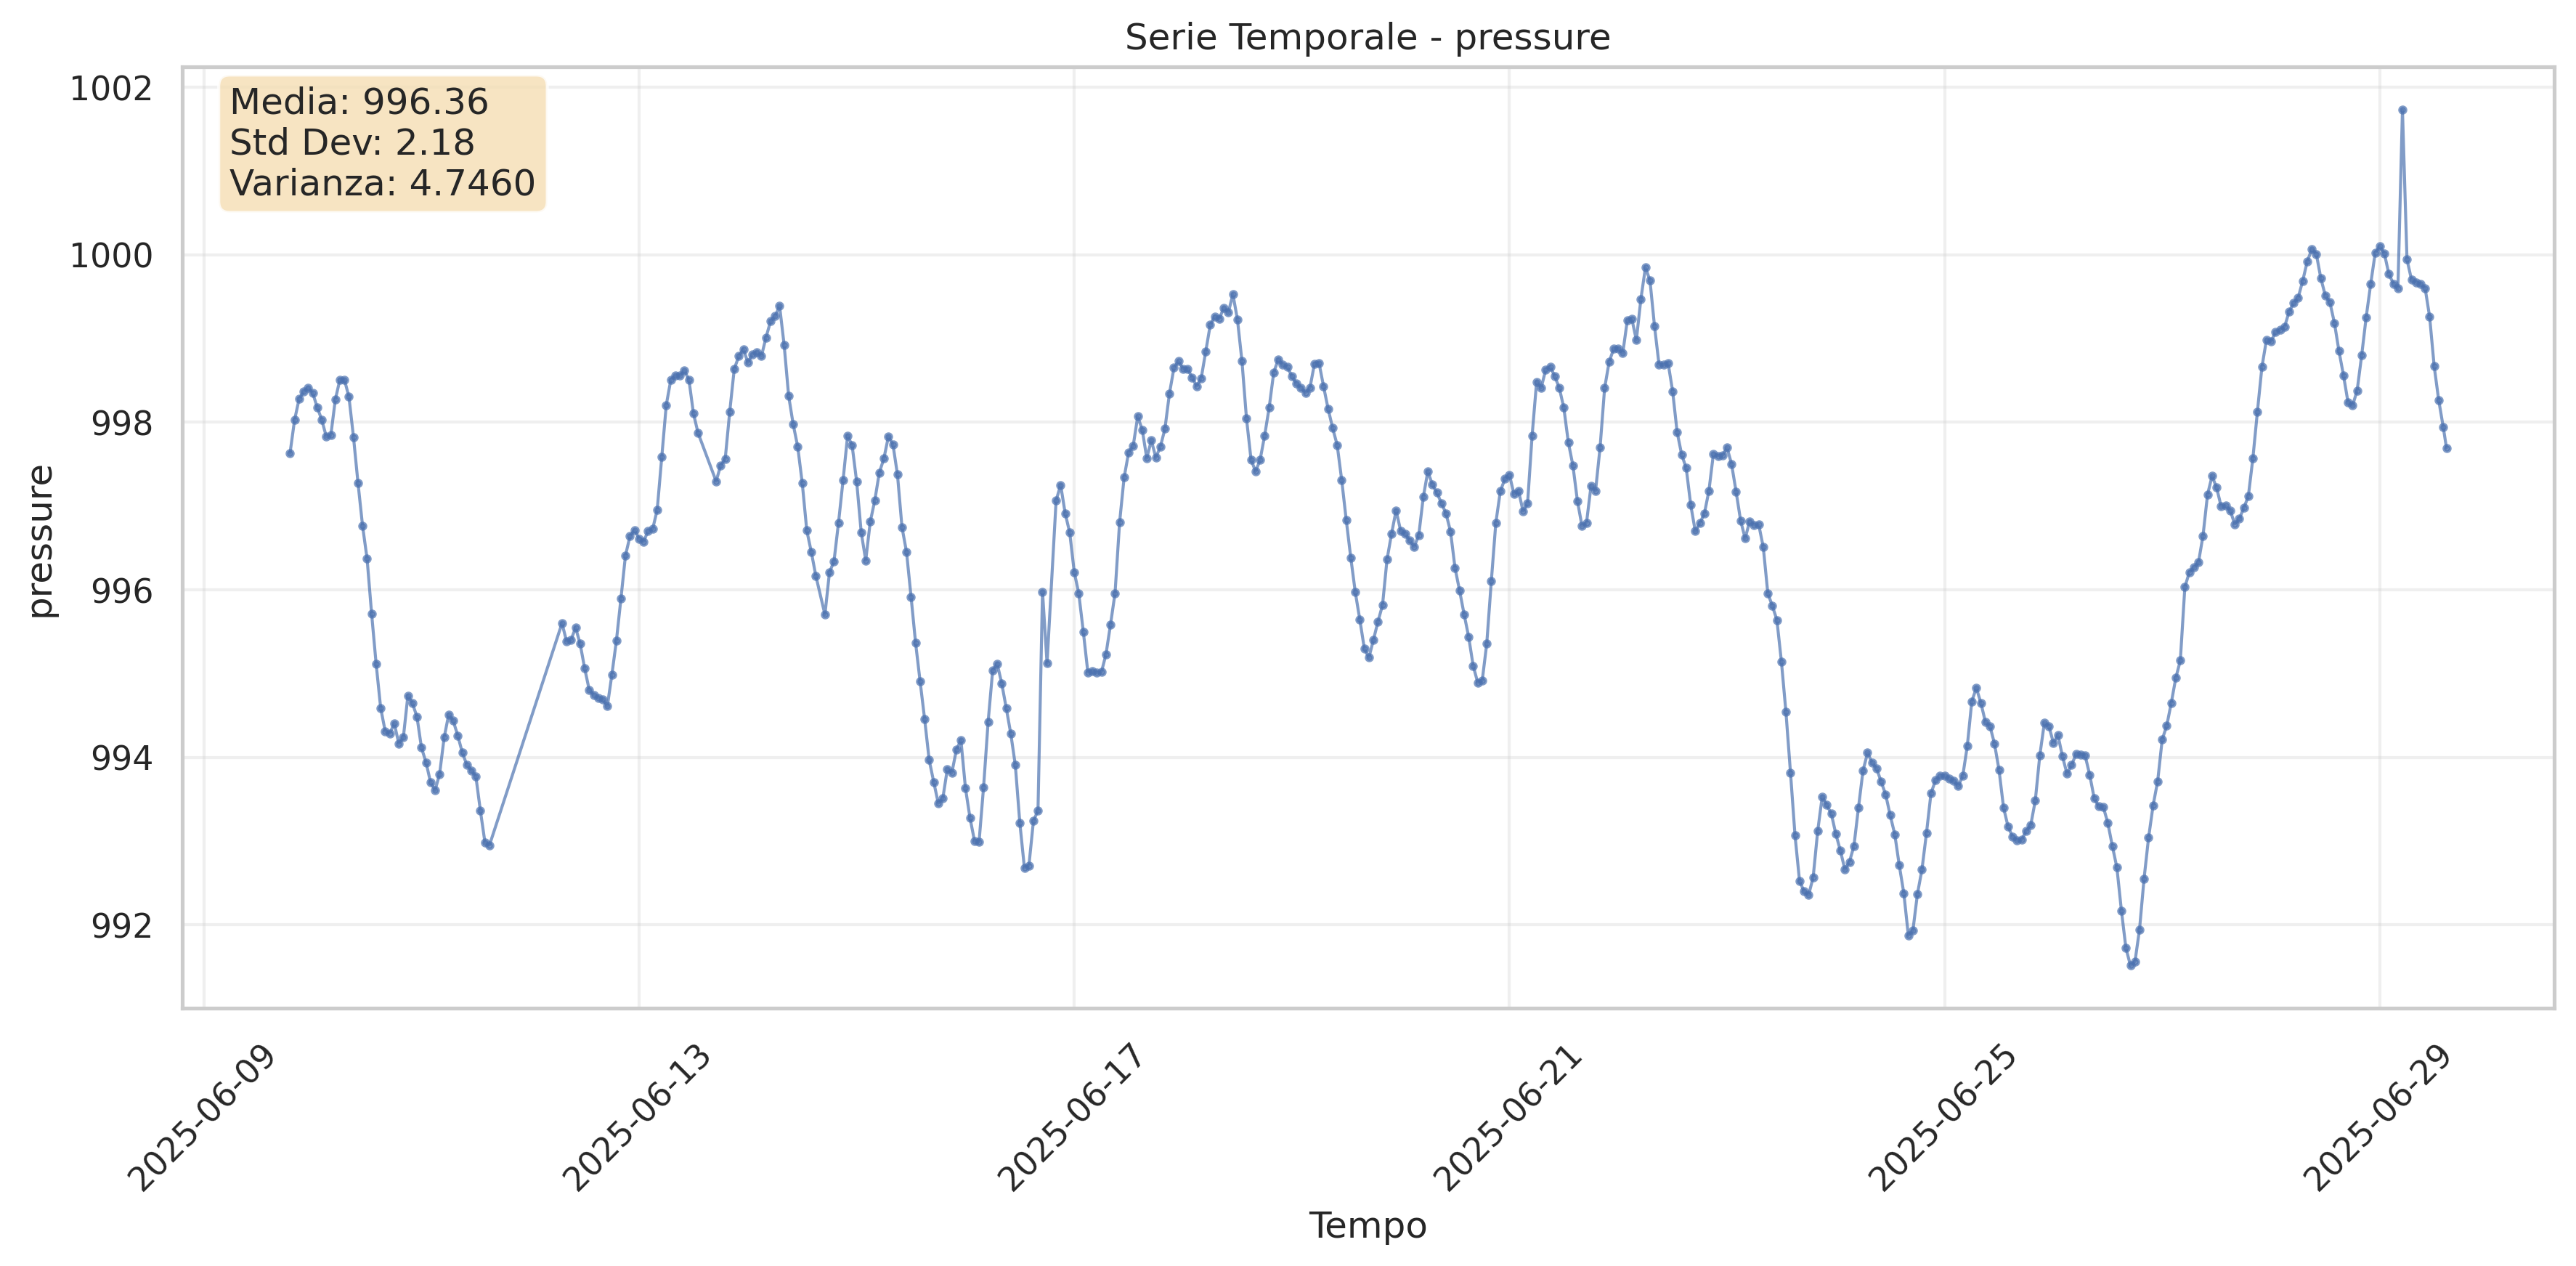
\includegraphics[width=\linewidth]{Figures/pressure_timeseries}
	\caption{Andamento temporale della pressione}
	\label{fig:pressure_timeseries}
\end{figure}

\begin{figure}[ht]\centering
	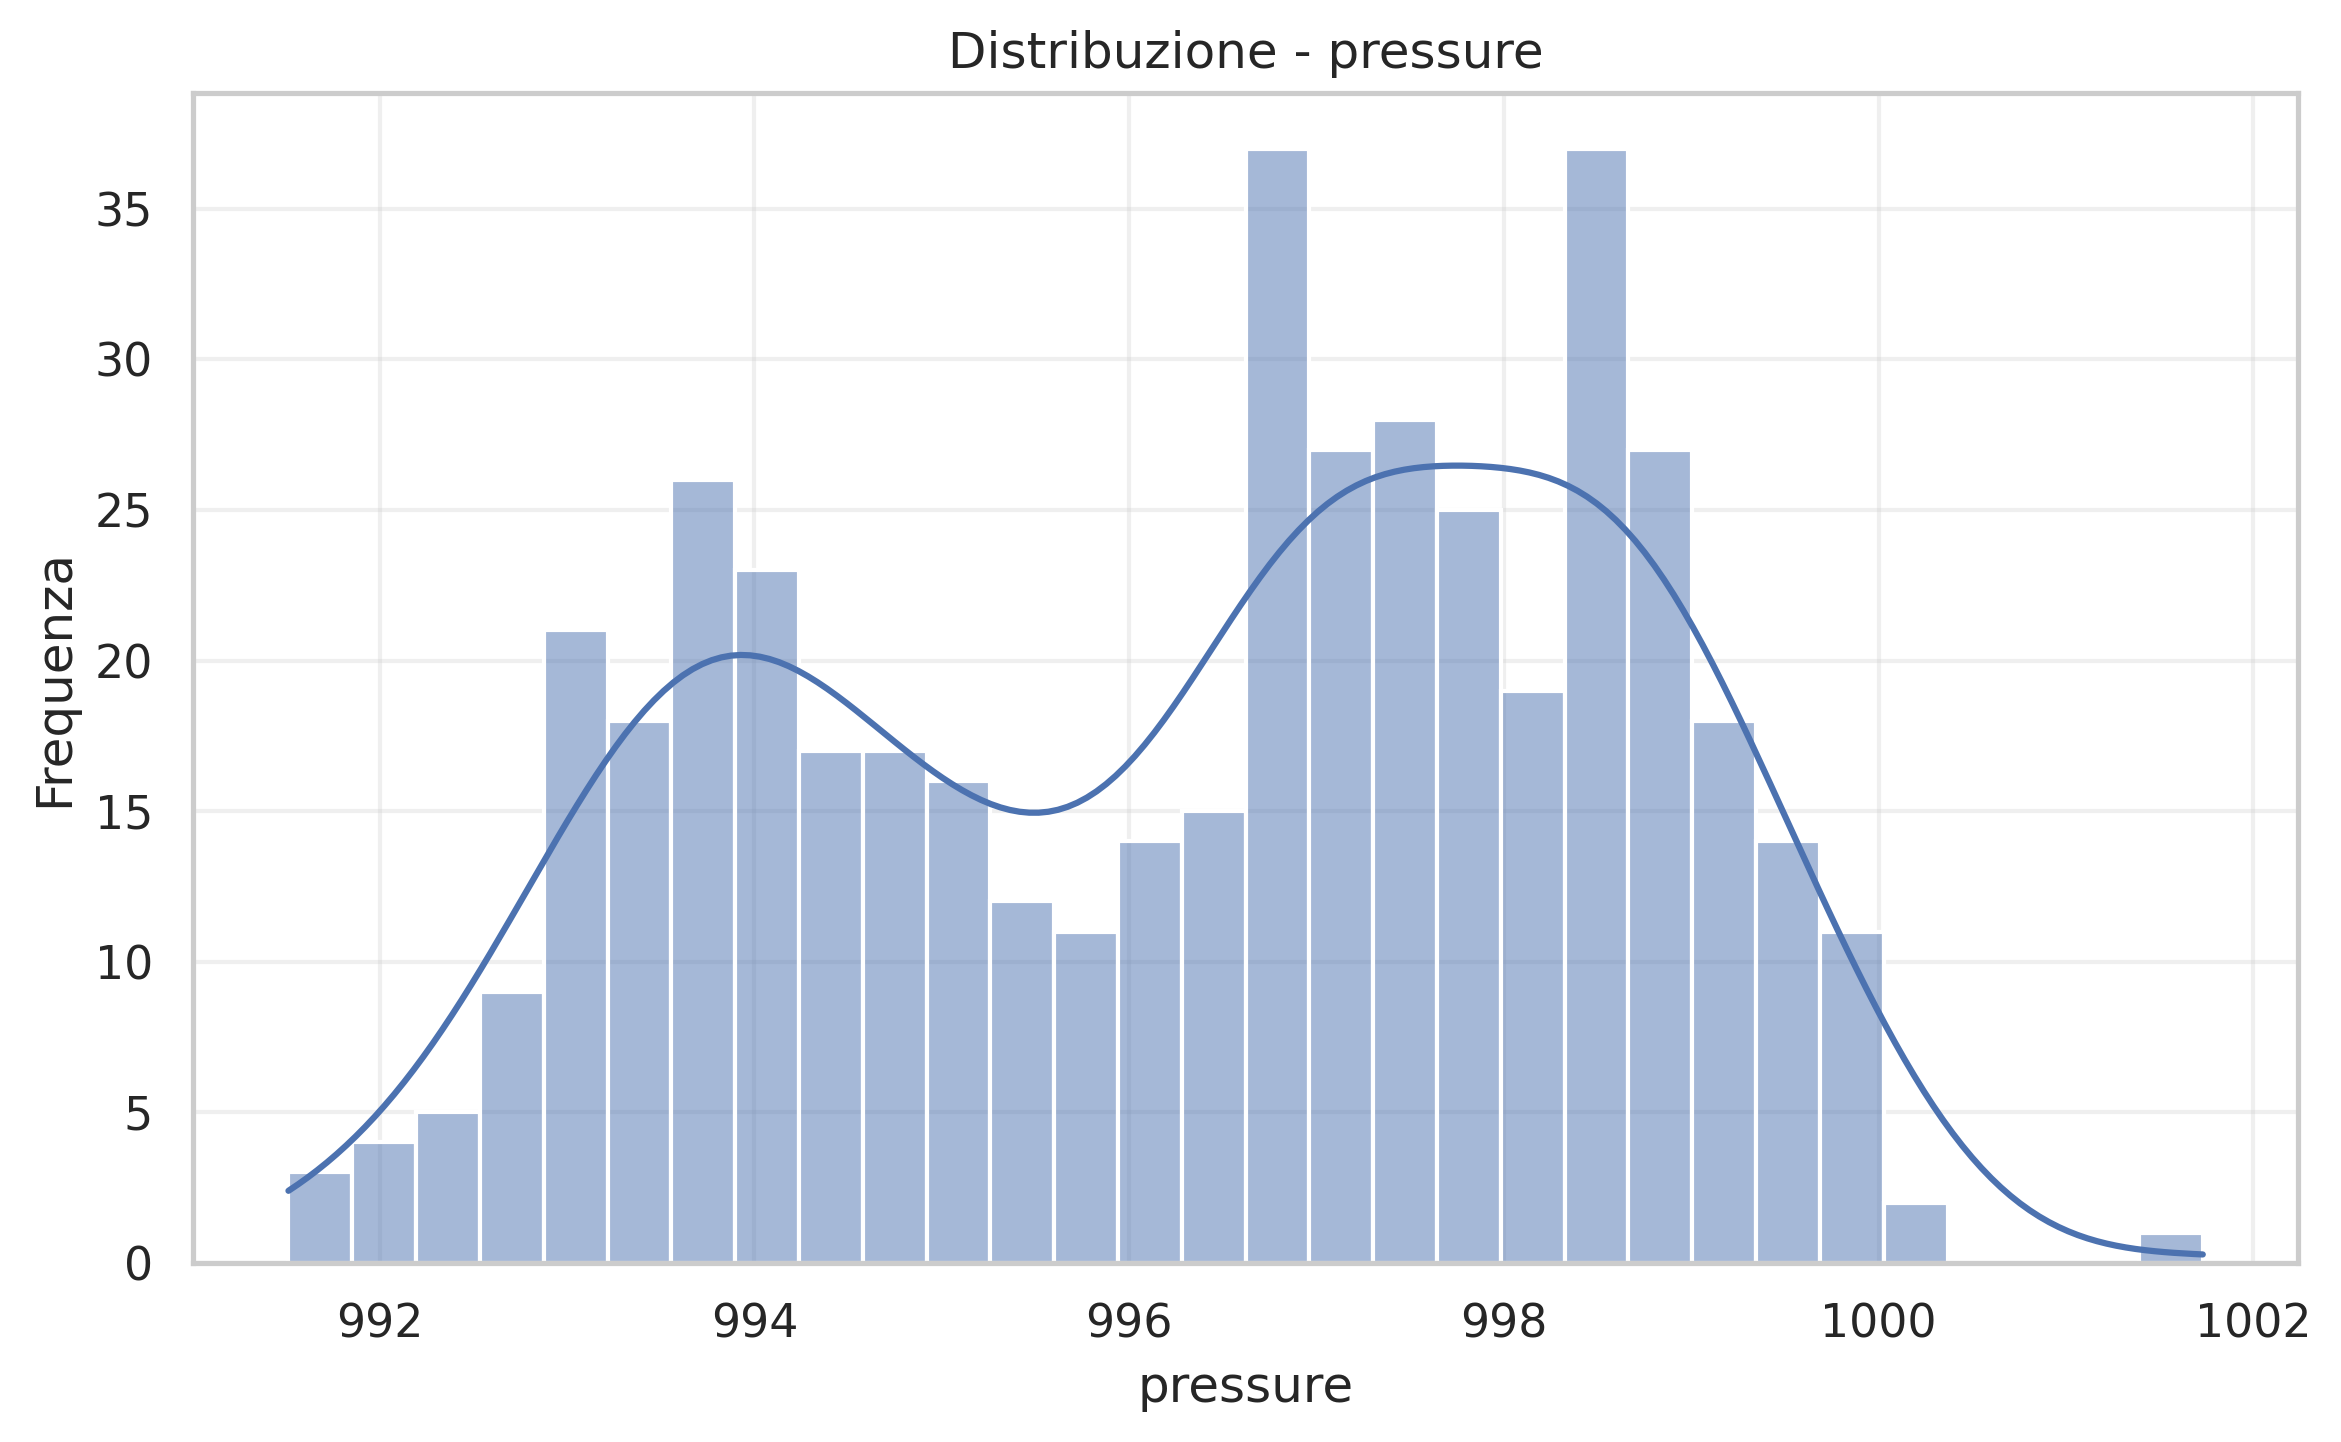
\includegraphics[width=\linewidth]{Figures/pressure_distribution}
	\caption{Distribuzione della pressione}
	\label{fig:press_dis}
\end{figure}

Per quanto riguarda l’umidità relativa (Figura~\ref{fig:humidity_timeseries}), i dati raccolti hanno mostrato comportamenti anomali, con letture prossime allo 0\% in condizioni di bassa umidità. Si ipotizza un malfunzionamento del sensore, probabilmente al di sotto di una soglia operativa minima. Per garantire l’affidabilità nell’addestramento del modello, tali valori sono stati corretti ponendo un limite inferiore al 20\%. I valori massimi si registrano tipicamente nelle ore precedenti all’alba, coerentemente con la ridotta temperatura dell’aria.

\begin{figure}[ht]\centering
	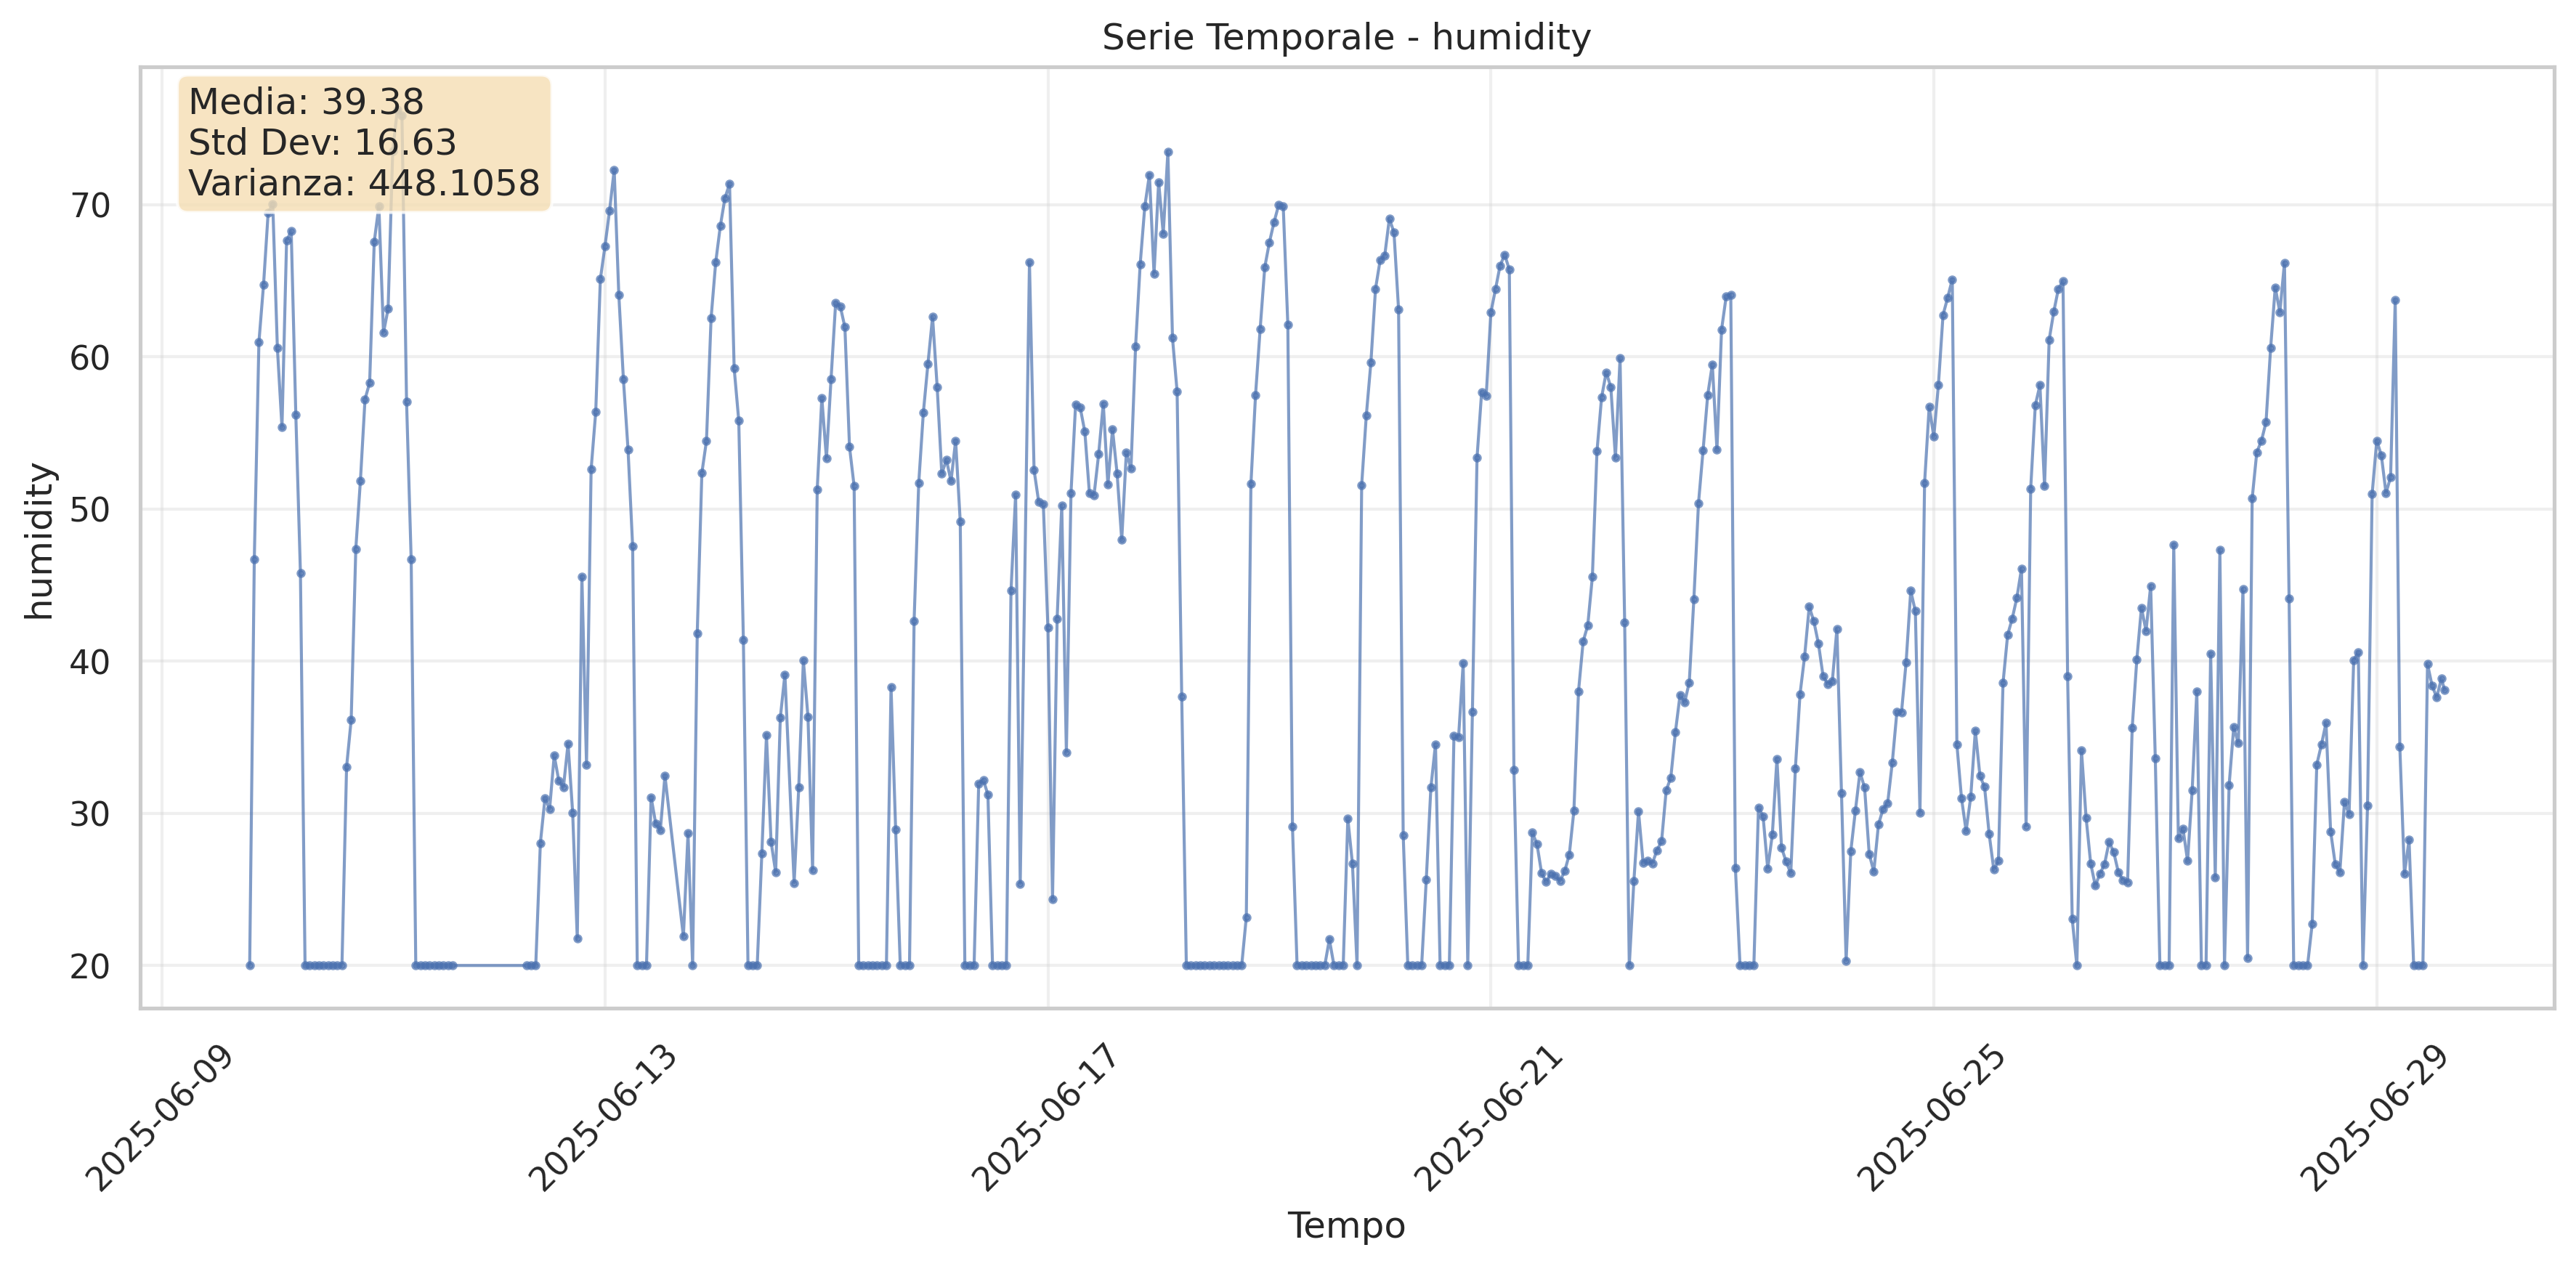
\includegraphics[width=\linewidth]{Figures/humidity_timeseries}
	\caption{Andamento temporale dell'umidità}
	\label{fig:humidity_timeseries}
\end{figure}

Il sensore ENS160 utilizza temperatura e umidità esterne per compensare i valori calcolati di \textit{equivalent CO\textsubscript{2}} (eCO\textsubscript{2}). Tuttavia, come mostrato in Figura~\ref{fig:ens160_timeseries}, le anomalie nei dati di umidità si riflettono in oscillazioni irrealistiche nella stima dell’eCO\textsubscript{2}.

\begin{figure}[ht]\centering
	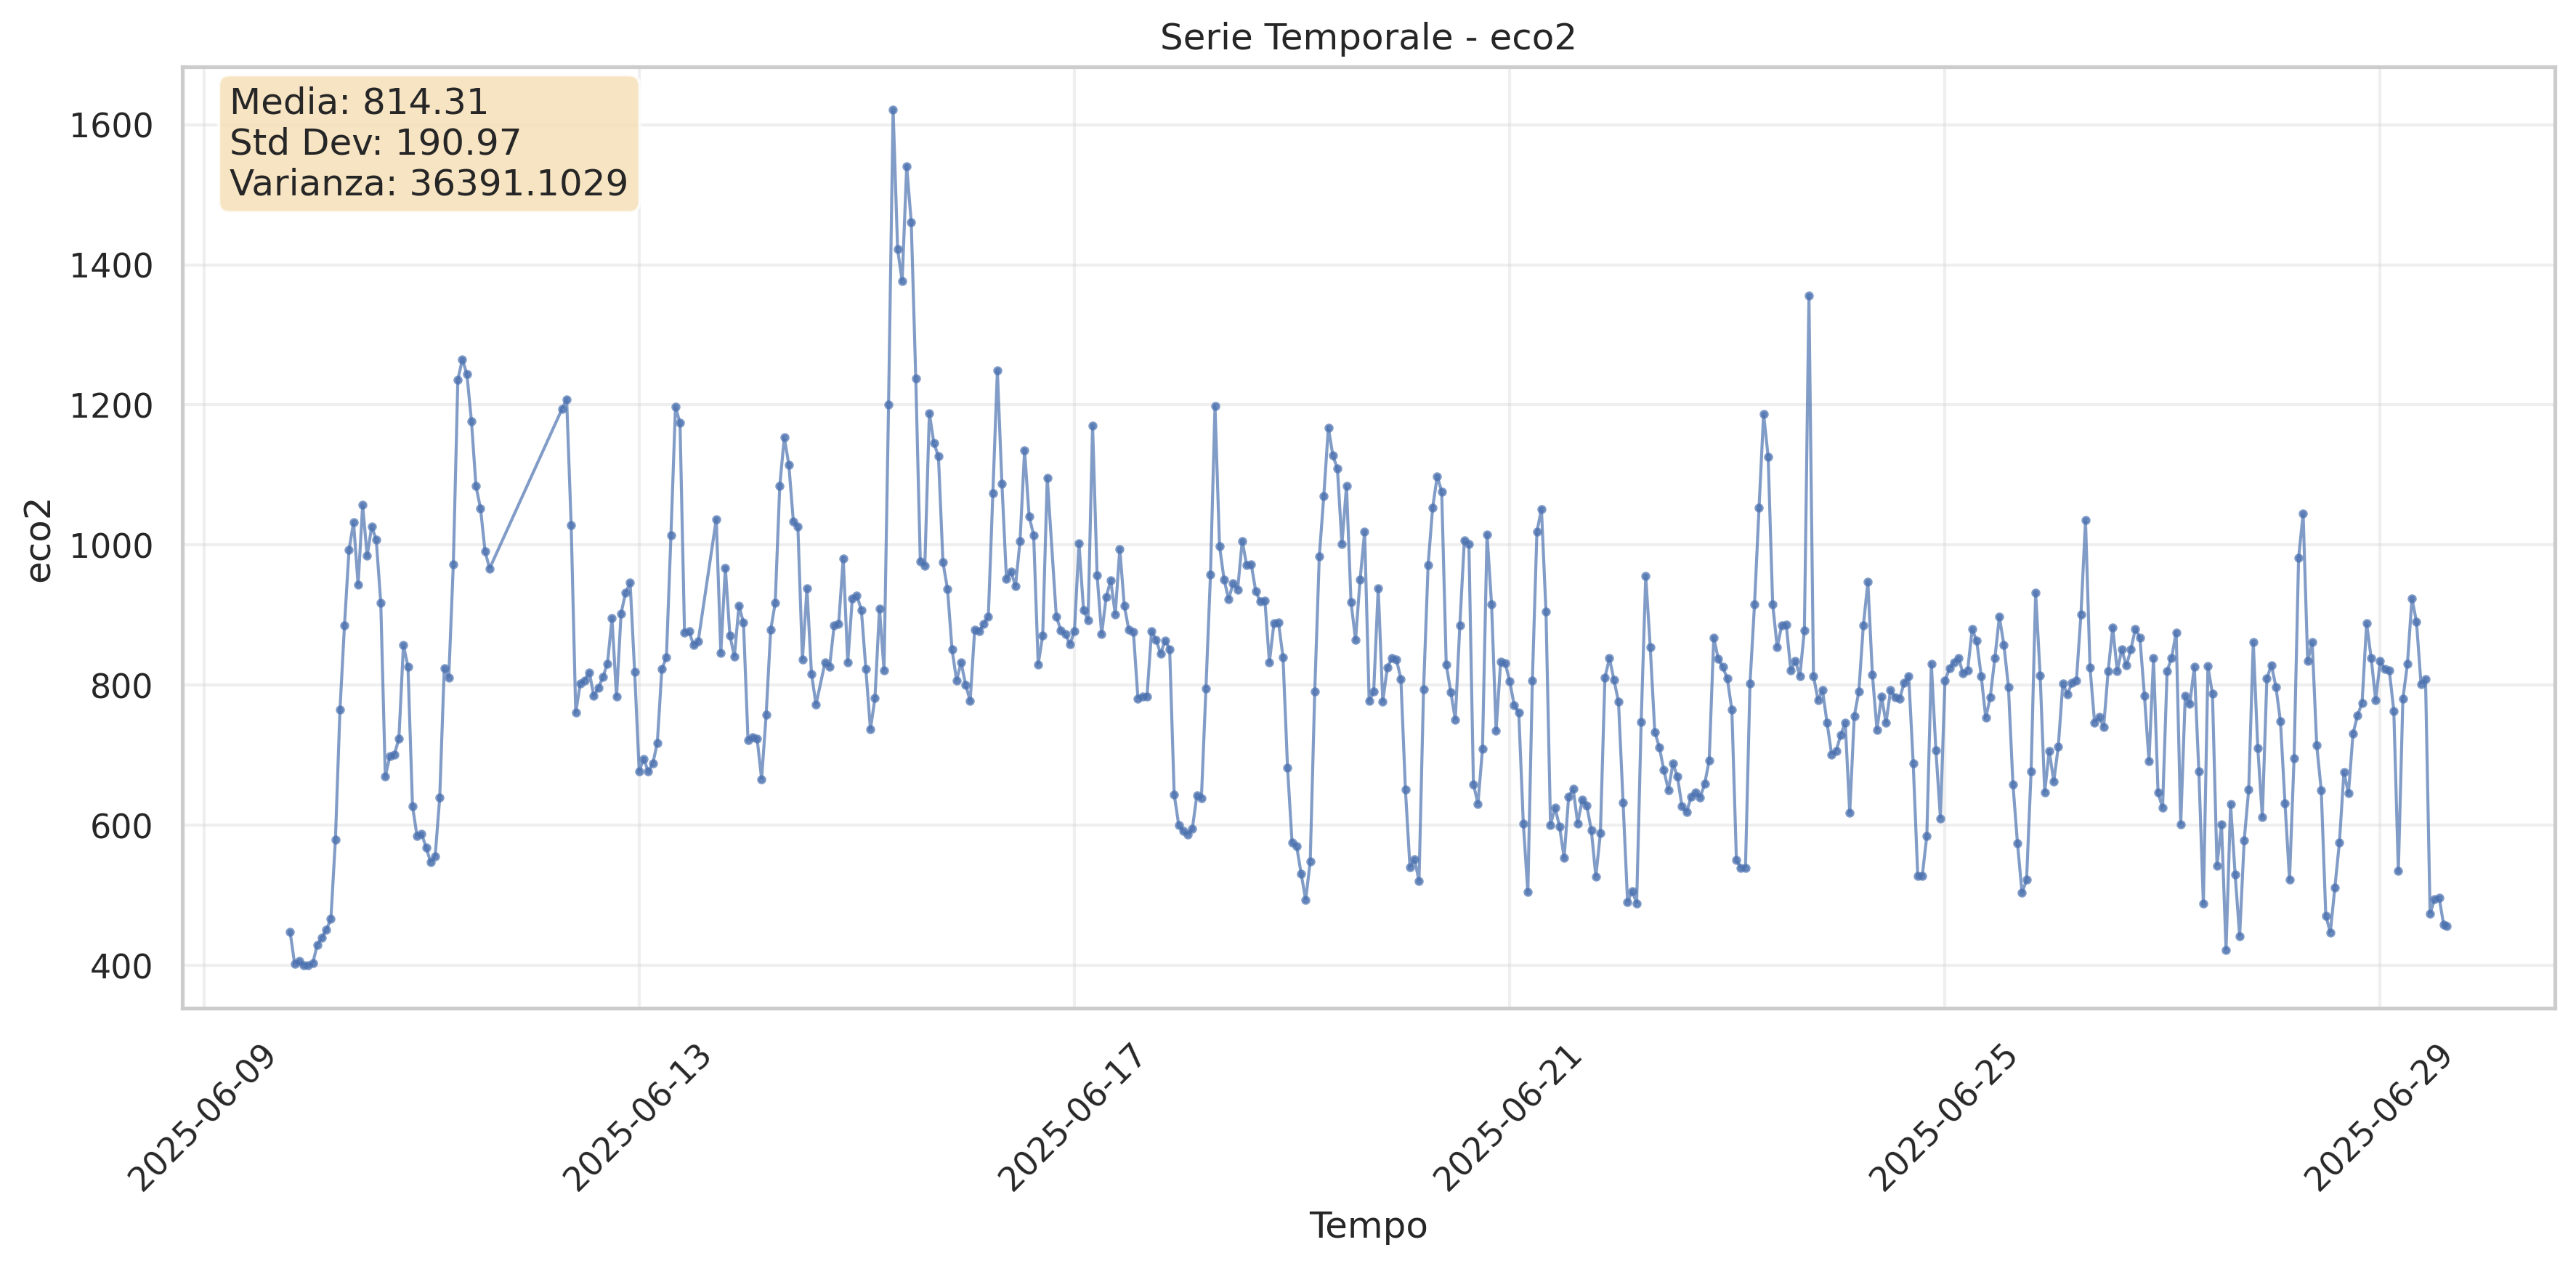
\includegraphics[width=\linewidth]{Figures/eco2_timeseries}
	\caption{Andamento temporale della eCO\textsubscript{2} stimata dal sensore ENS160}
	\label{fig:ens160_timeseries}
\end{figure}

In contrasto, il sensore MH-Z19B fornisce misurazioni dirette della concentrazione di CO\textsubscript{2}, mostrate in Figura~\ref{fig:mhz19b_timeseries}, con valori generalmente compresi tra 400 e 500 ppm. La distribuzione (Figura~\ref{fig:mhz19b_distribution}) conferma l’attendibilità delle misure, con una distribuzione normale centrata nel range atteso.

\begin{figure}[ht]\centering
	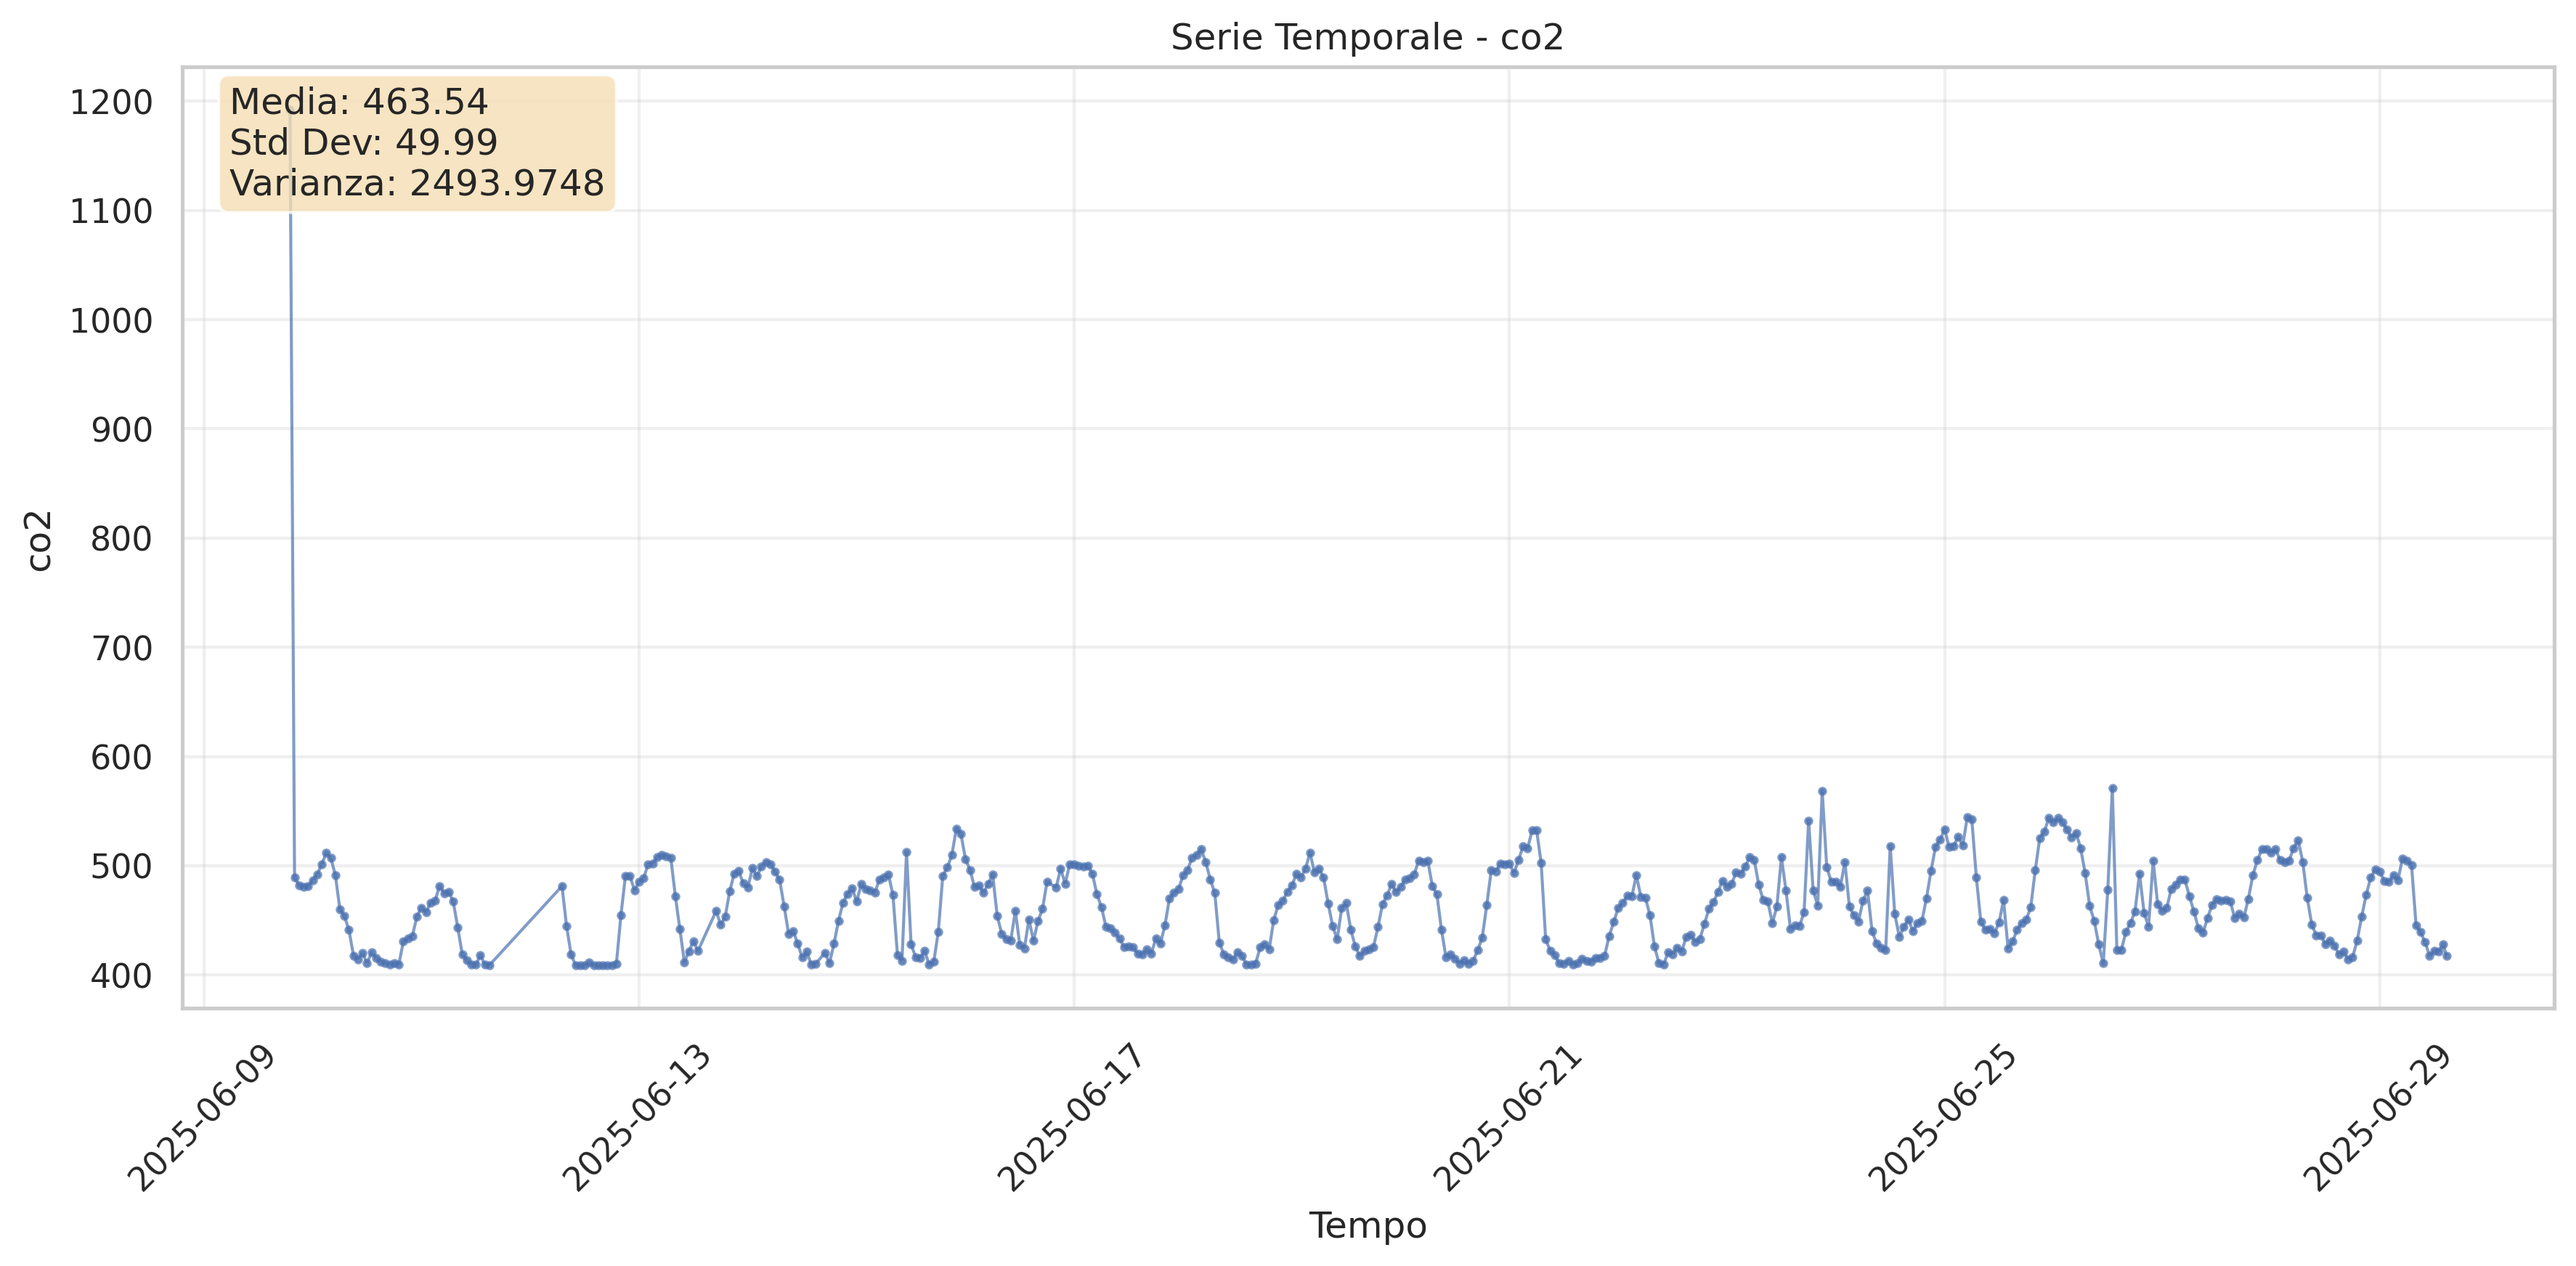
\includegraphics[width=\linewidth]{Figures/co2_timeseries}
	\caption{Andamento temporale della CO\textsubscript{2} rilevata dal sensore MH-Z19B}
	\label{fig:mhz19b_timeseries}
\end{figure}

\begin{figure}[ht]\centering
	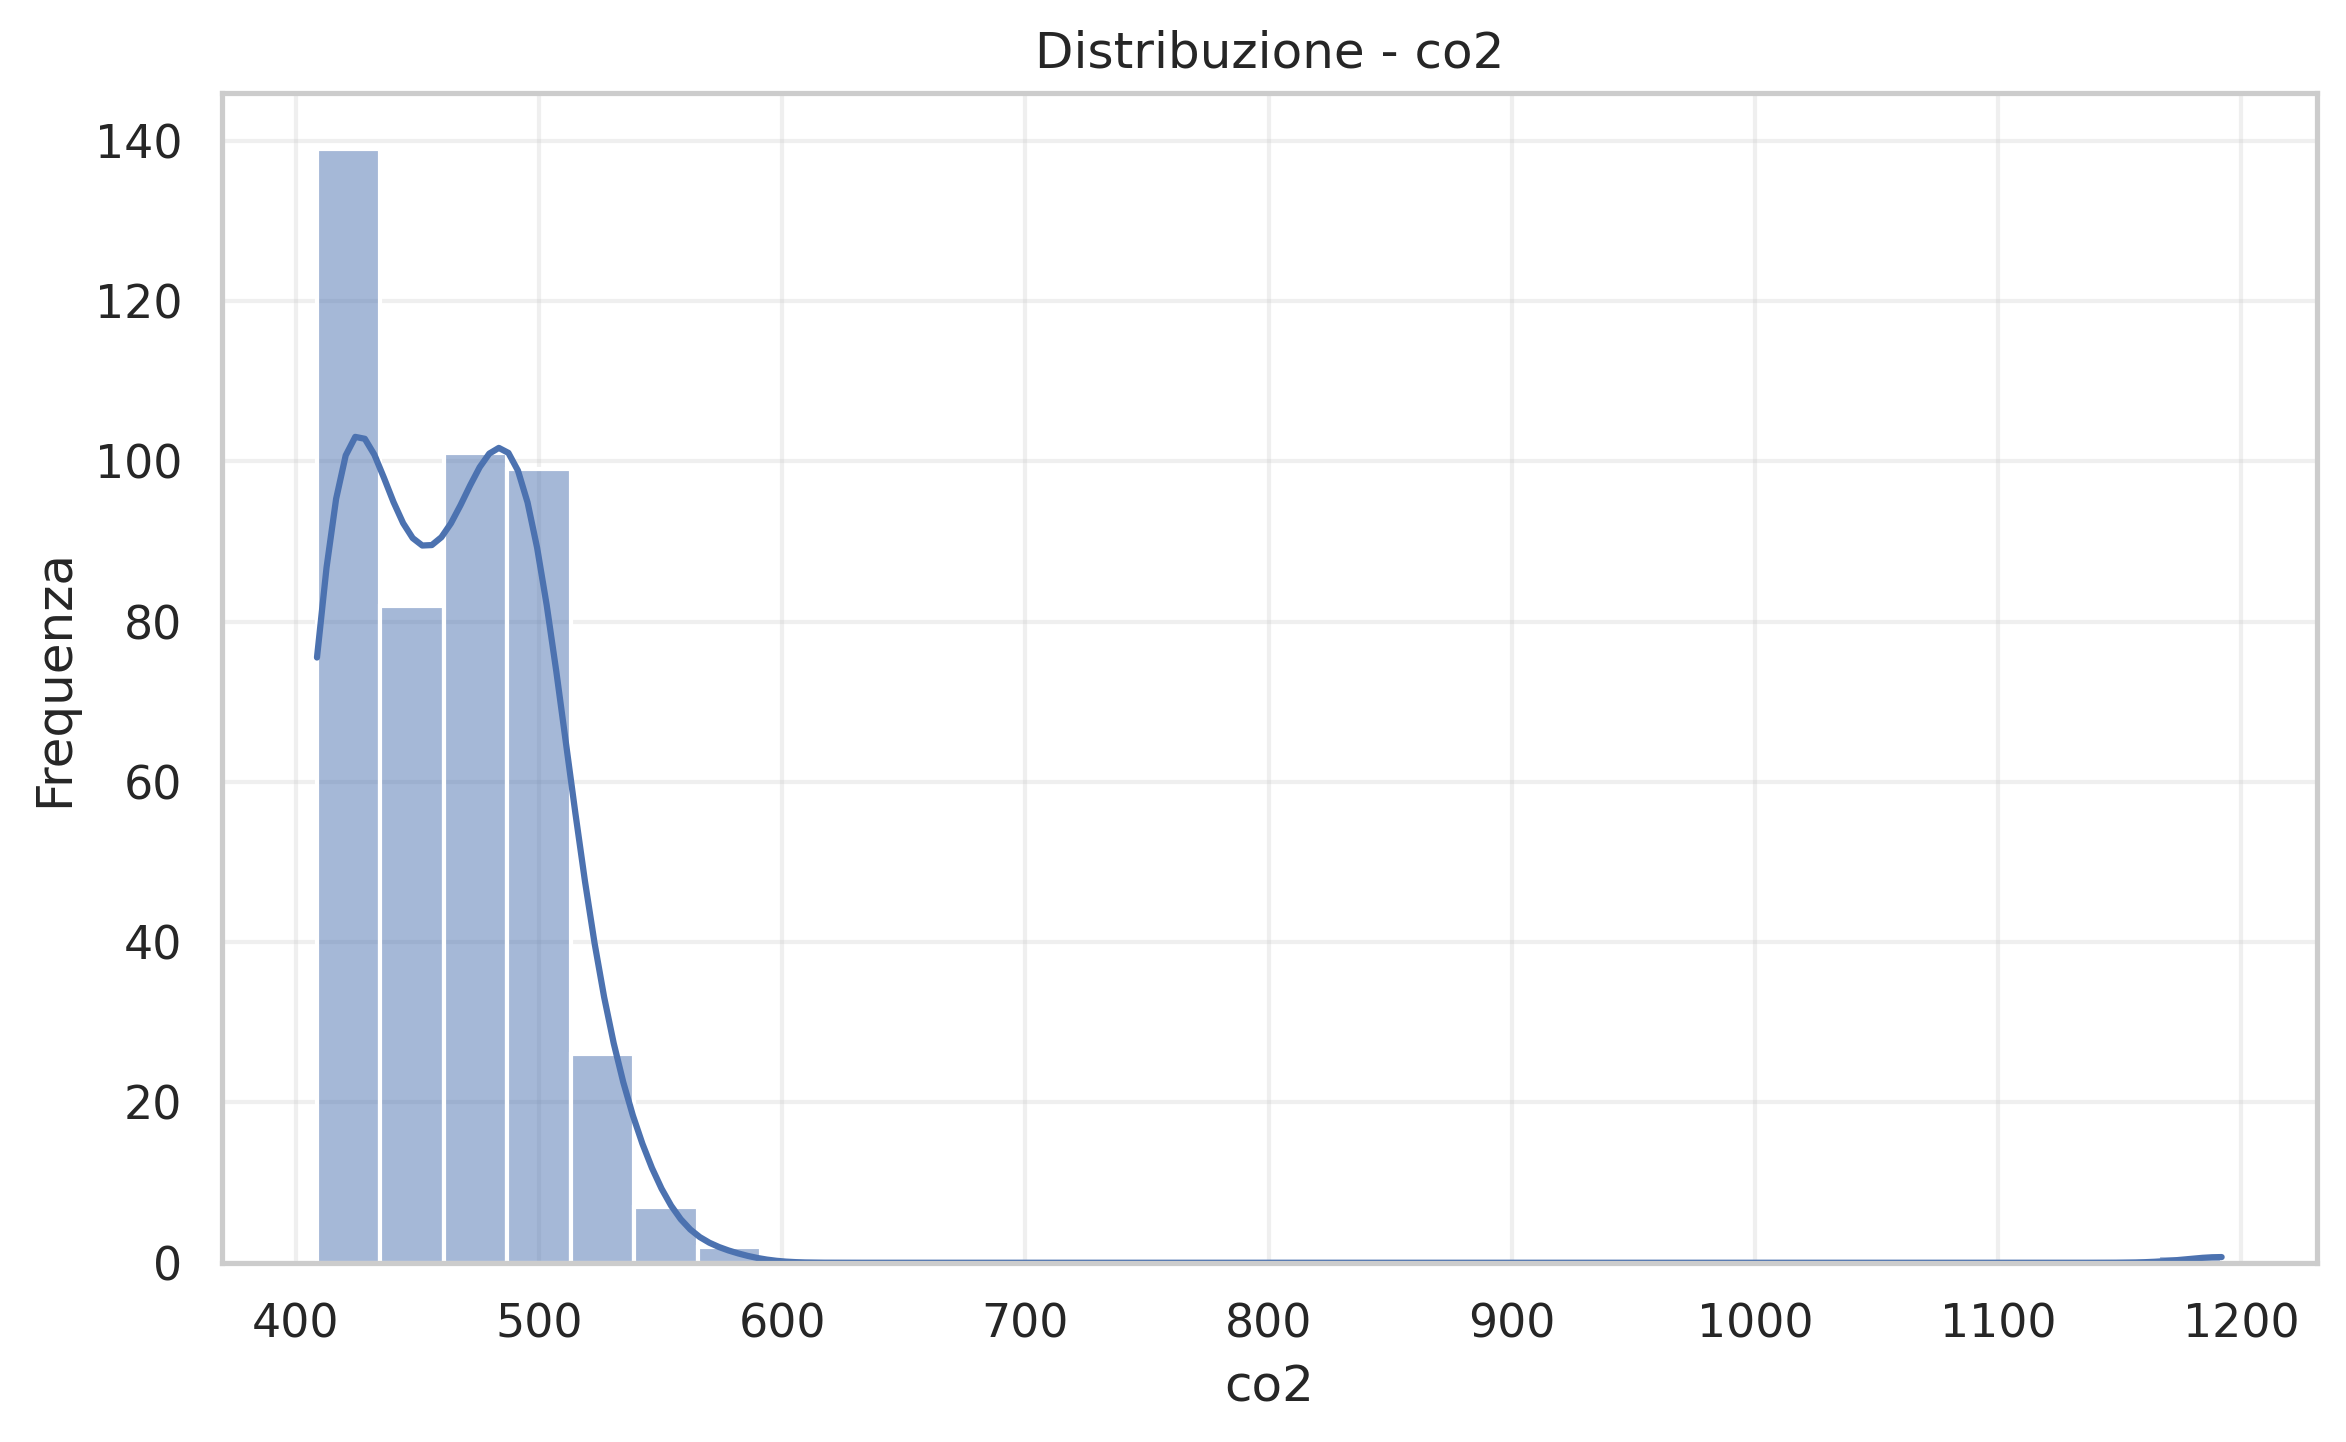
\includegraphics[width=\linewidth]{Figures/co2_distribution}
	\caption{Distribuzione della CO\textsubscript{2} rilevata dal sensore MH-Z19B}
	\label{fig:mhz19b_distribution}
\end{figure}

I valori di particolato (Figura~\ref{fig:pm2p5_timeseries}) mostrano picchi attribuibili a fenomeni locali, come la combustione di rami ed erba nelle campagne marchigiane. Di particolare rilievo è l’incremento rilevato il 15 giugno 2025, attribuito al trasporto transatlantico degli inquinanti derivanti dagli incendi in Canada. 

\begin{figure}[ht]\centering
	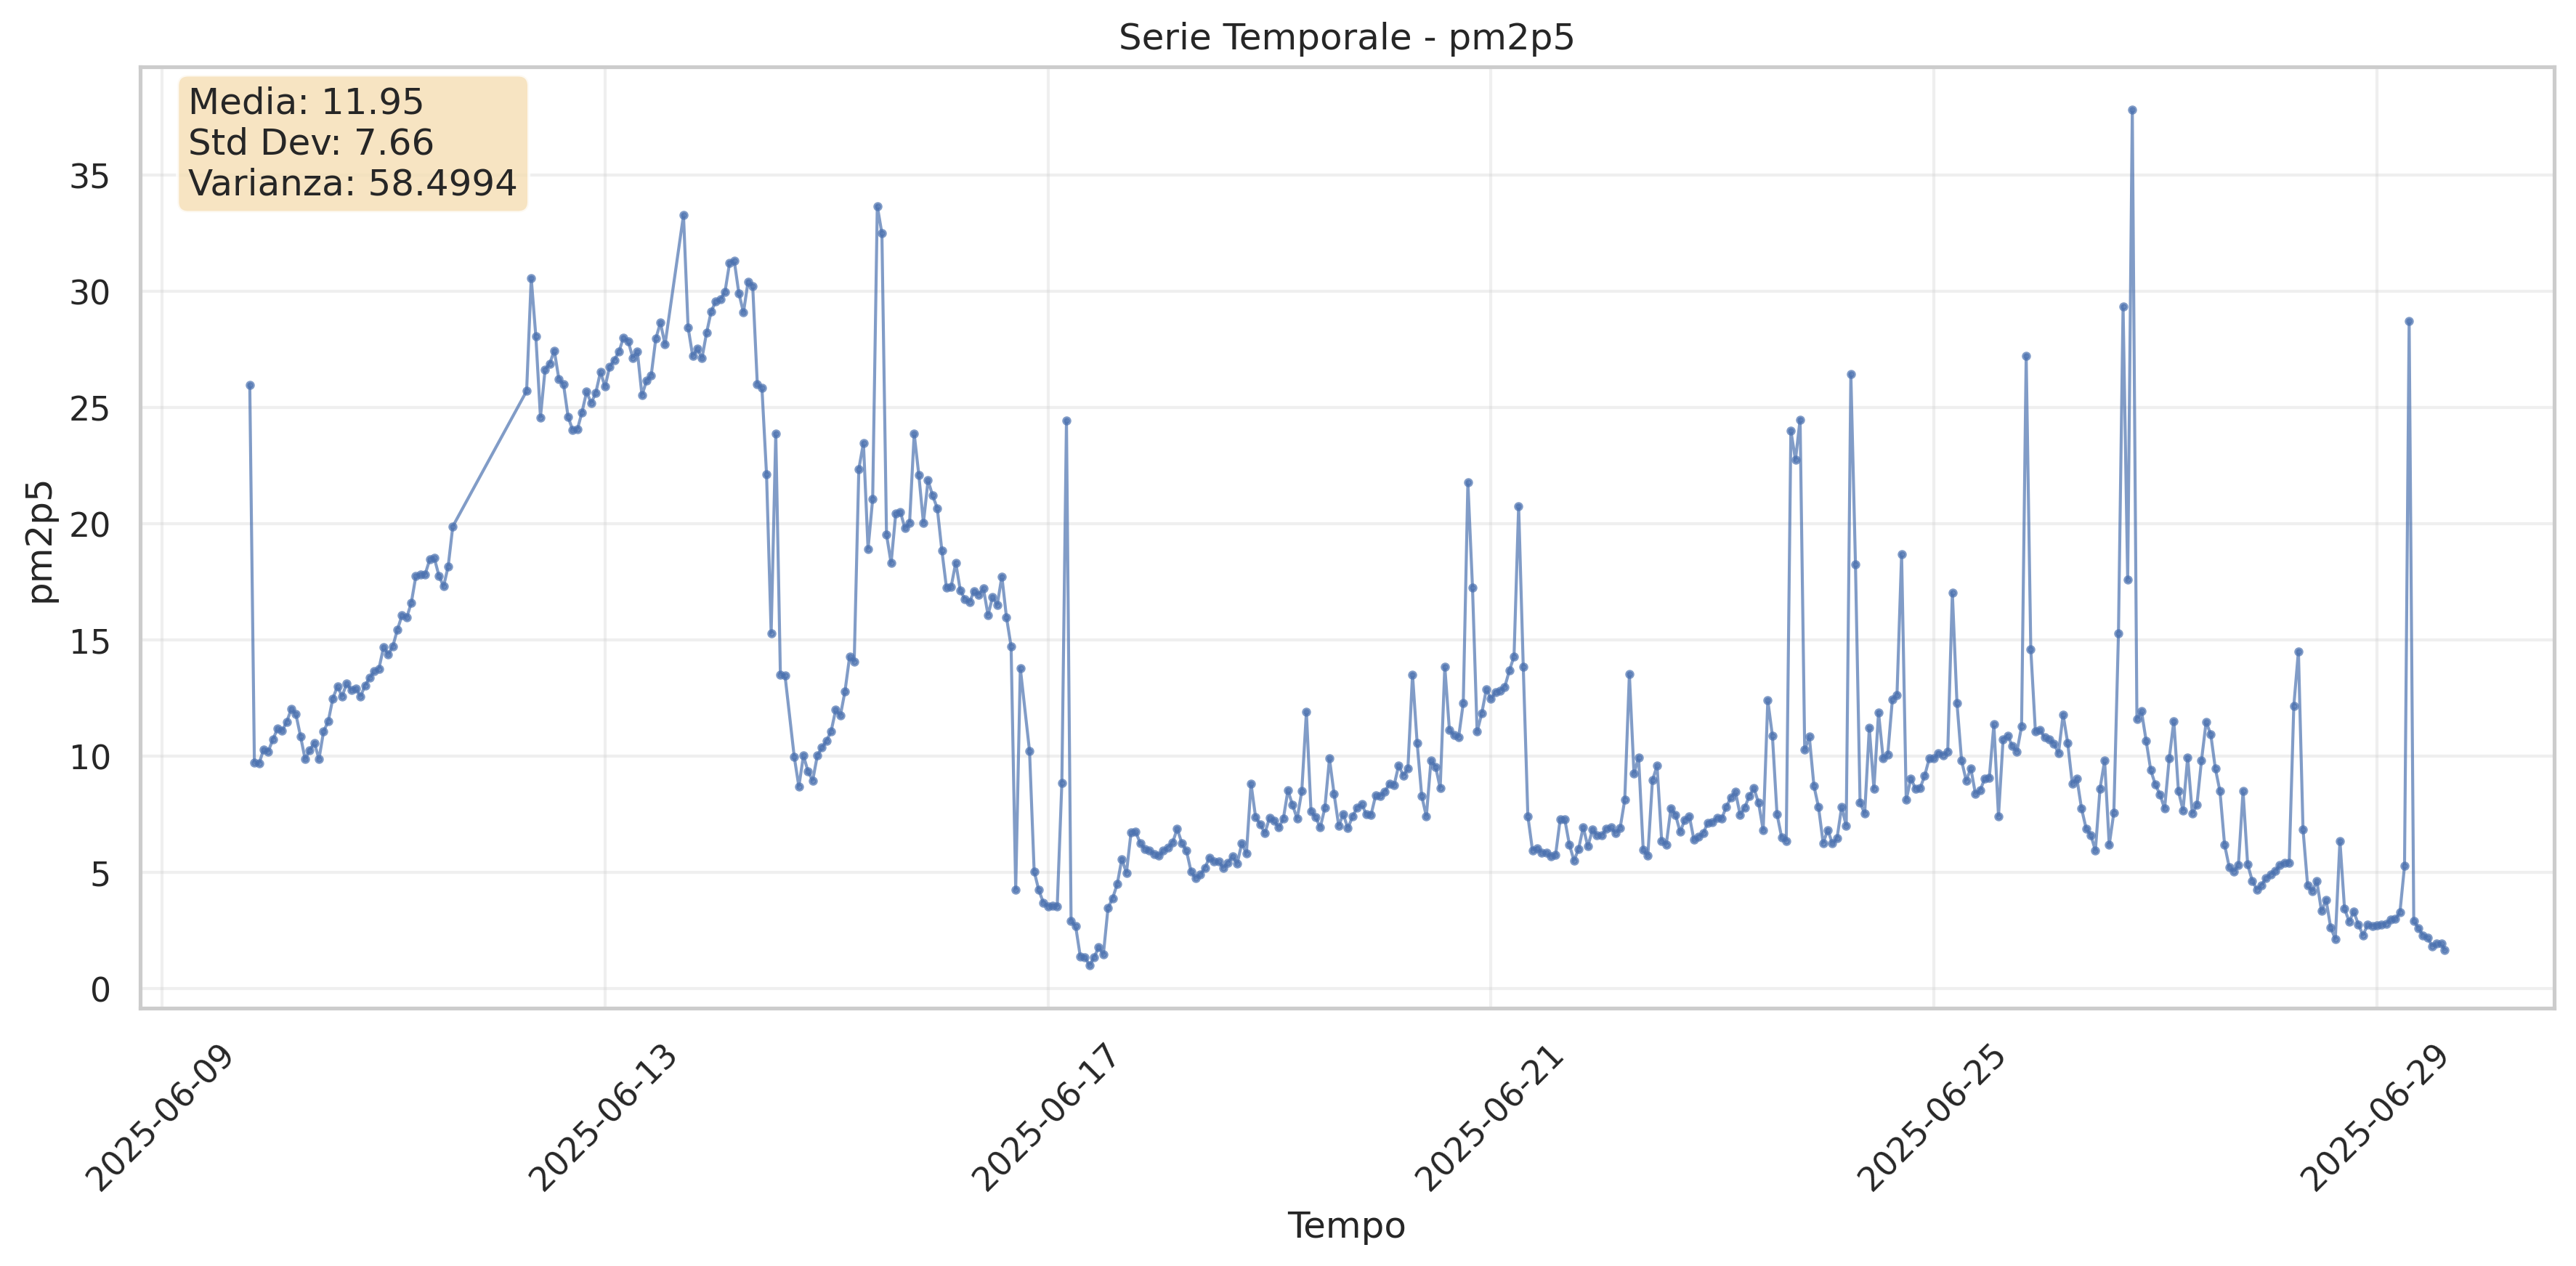
\includegraphics[width=\linewidth]{Figures/pm2p5_timeseries}
	\caption{Andamento temporale del particolato PM2.5}
	\label{fig:pm2p5_timeseries}
\end{figure}


Pur avendo registrato anche PM1.0 e PM4.0, l’attenzione principale è rivolta a PM2.5 e PM10 (Figura~\ref{fig:pm10p0_timeseries}), che rappresentano le frazioni più rilevanti dal punto di vista sanitario. Come noto, PM2.5 include anche le particelle PM1.0, mentre PM10 comprende tutte le classi inferiori.

\begin{figure}[ht]\centering
	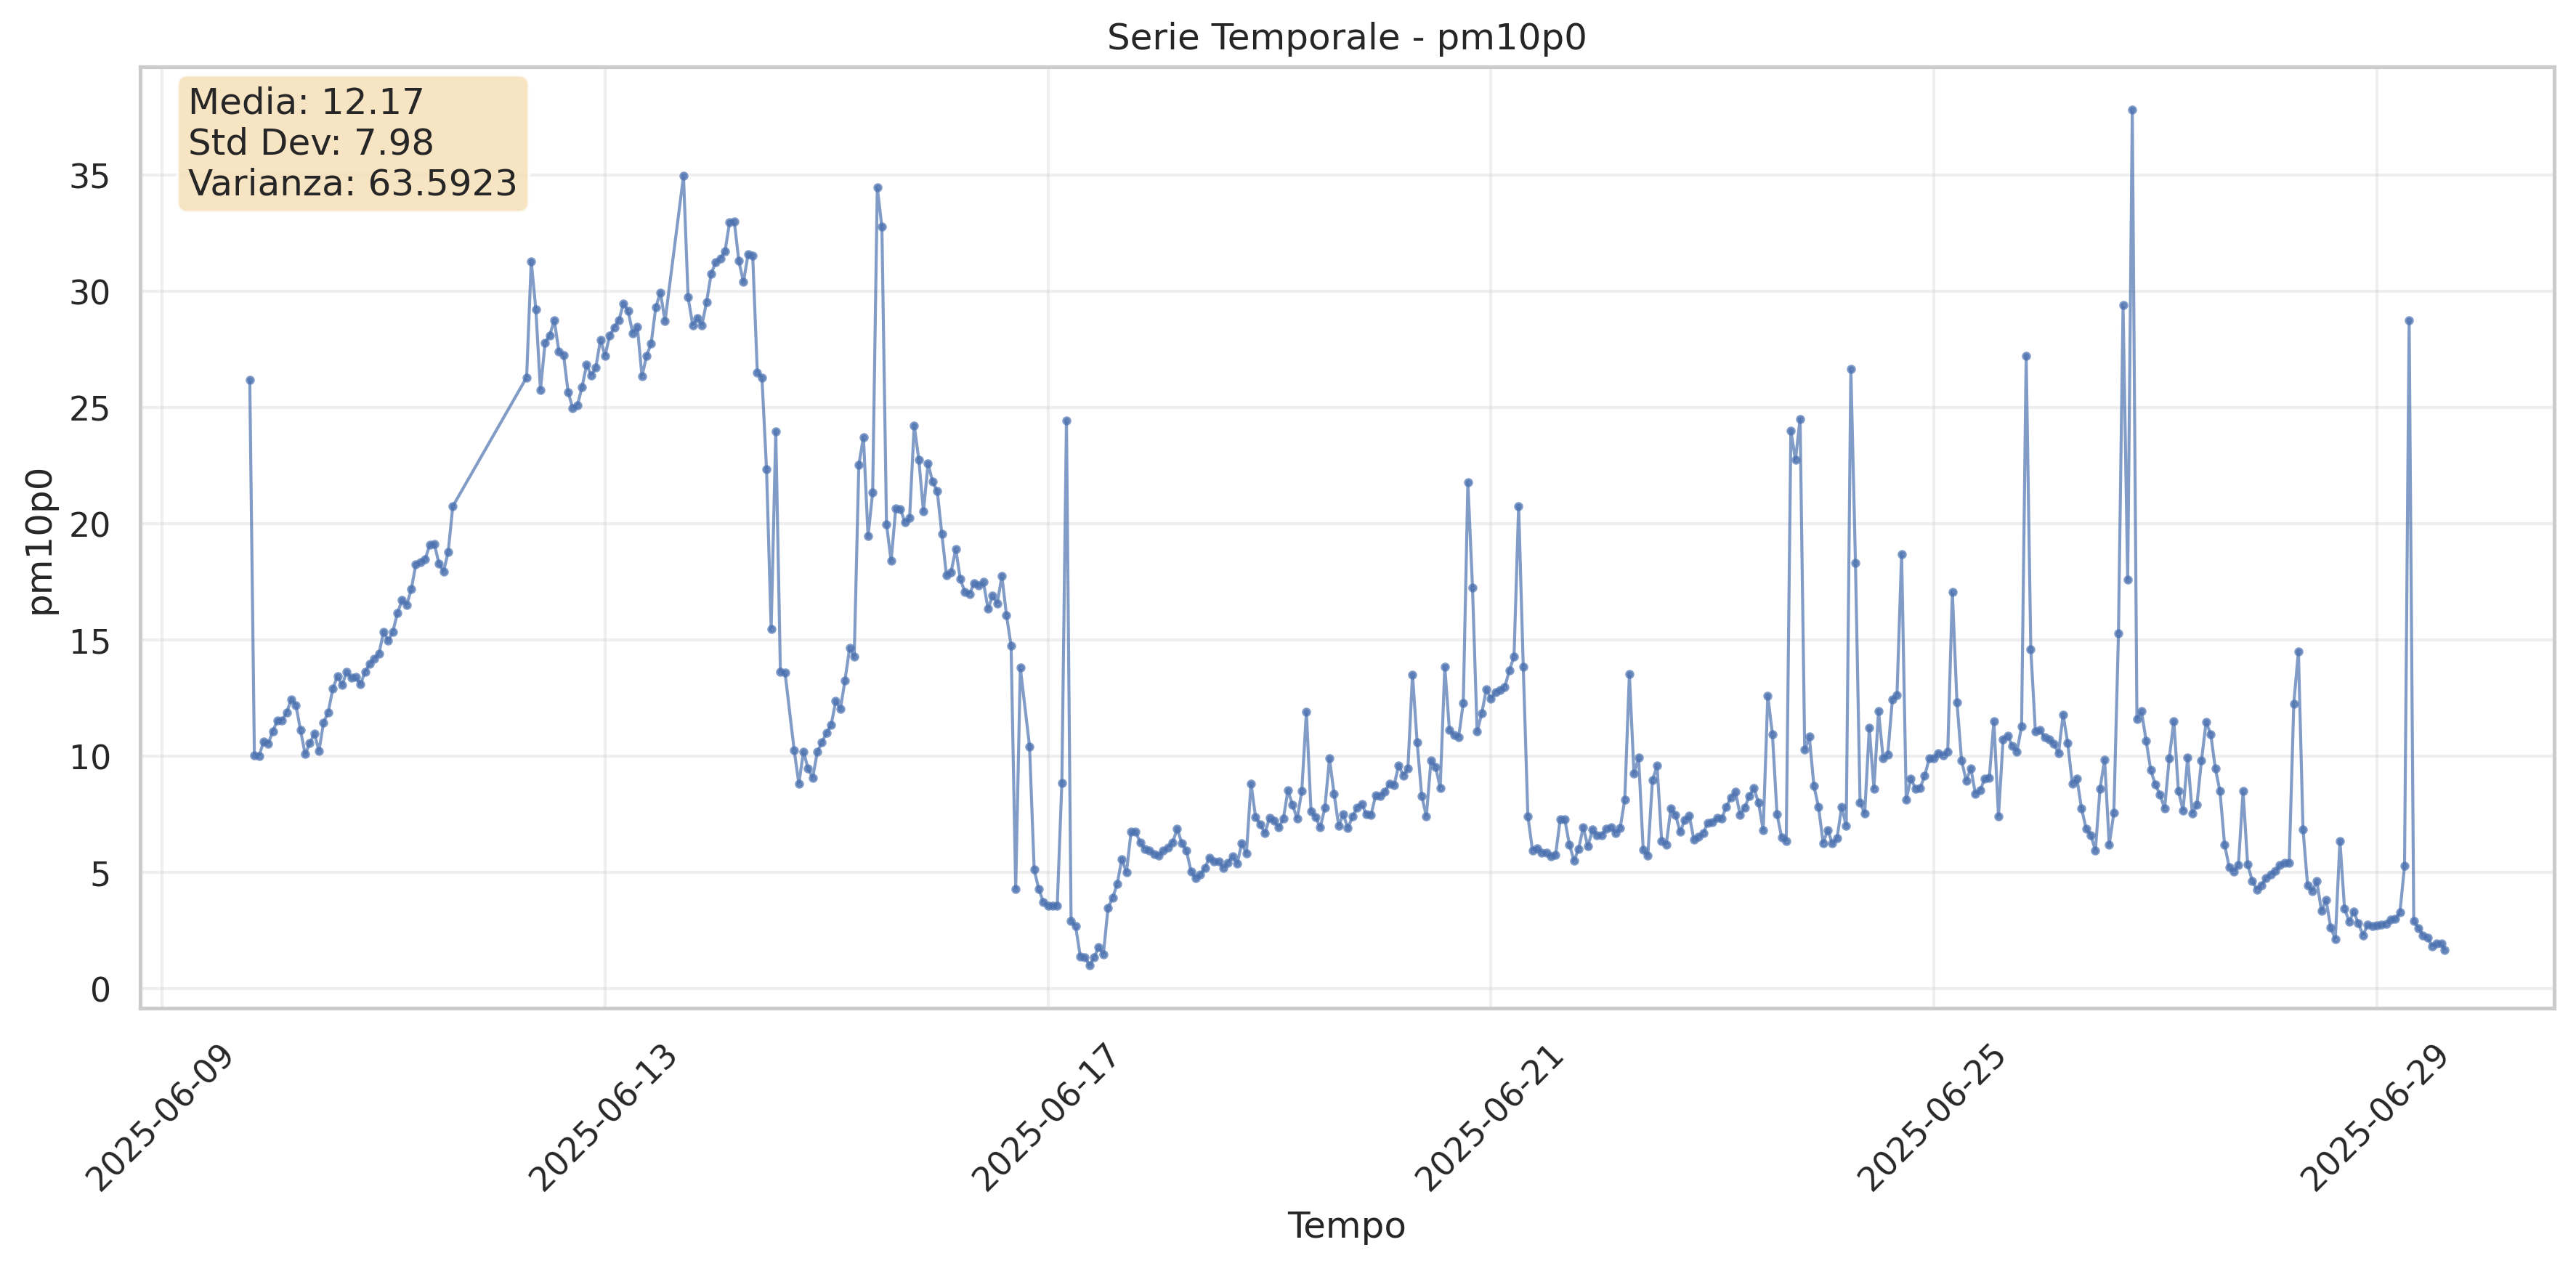
\includegraphics[width=\linewidth]{Figures/pm10p0_timeseries}
	\caption{Andamento temporale del particolato PM10}
	\label{fig:pm10p0_timeseries}
\end{figure}

Infine, l’andamento dei TVOC rilevati dal sensore ENS160 (Figura~\ref{fig:tvoc_timeseries}) evidenzia incrementi in corrispondenza degli eventi sopra descritti. A differenza della eCO\textsubscript{2}, il segnale dei TVOC non è compensato in base all’umidità, e pertanto fornisce una rappresentazione più robusta delle variazioni di composti organici volatili in atmosfera.

\begin{figure}[ht]\centering
	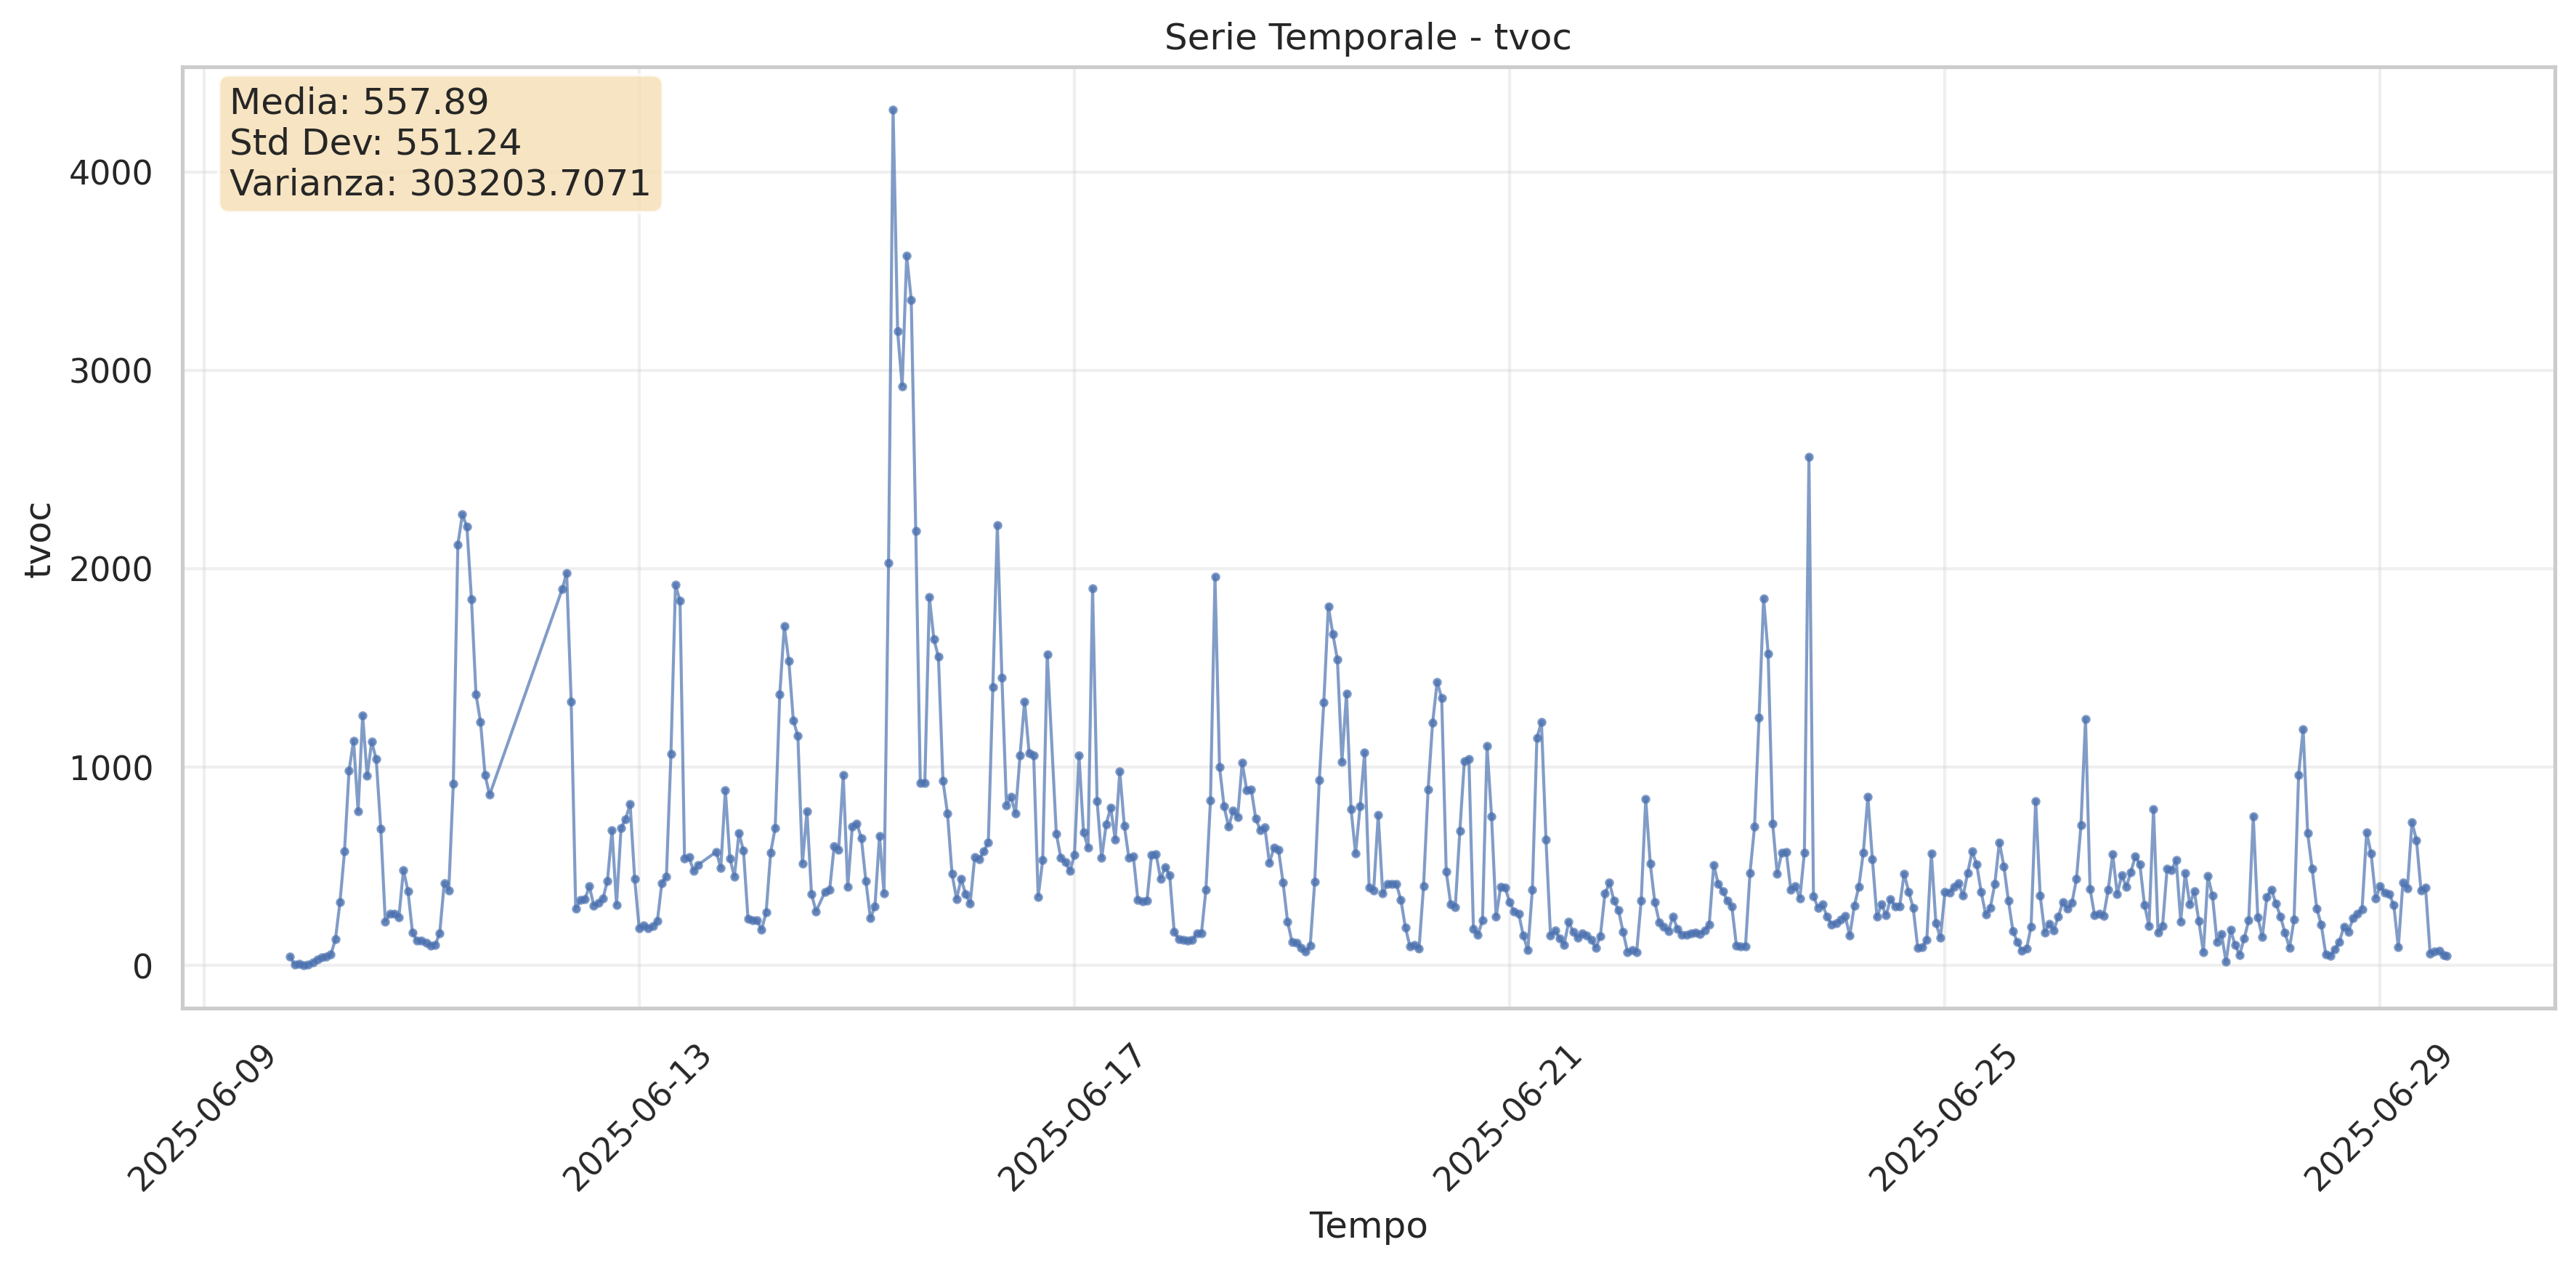
\includegraphics[width=\linewidth]{Figures/tvoc_timeseries}
	\caption{Andamento temporale dei composti organici volatili totali (TVOC)}
	\label{fig:tvoc_timeseries}
\end{figure}

\section{Il modello di Machine Learning}
\lipsum
\section{Conclusioni}
\lipsum
%----------------------------------------------------------------------------------------
%	REFERENCE LIST
%----------------------------------------------------------------------------------------

\phantomsection
\bibliographystyle{unsrt}
\bibliography{sample.bib}

%----------------------------------------------------------------------------------------

\end{document}
